

%\documentclass[a4paper,twoside,11pt]{report}
\documentclass[a4paper, 11pt]{book}

\usepackage[small,bf]{caption}

% for images
\usepackage{graphicx}
\usepackage{subfig}

% to skip space but not indent for paragraph
\usepackage{parskip}

% for jumping to correct location from editor
%\usepackage{pdfsync}

% for UTF-8 support
\usepackage[utf8]{inputenc}

% for sideway tables
%\usepackage{rotating}

% for math
\usepackage{amsmath}

% for image wrapping
%\usepackage{wrapfig}

% for algorithms
\usepackage{algorithm}
\usepackage{algorithmic}

% for nice sitation references
\usepackage{natbib}

% for fancy headers
\usepackage{fancyhdr}
\pagestyle{fancy}
\renewcommand{\chaptermark}[1]{\markboth{\thechapter.\ #1}{}}
\usepackage{calc} \fancyheadoffset[LE,RO]{\marginparsep+\marginparwidth} \renewcommand{\chaptermark}[1]{\markboth{#1}{}} \renewcommand{\sectionmark}[1]{\markright{\thesection\ #1}} \fancyhf{}
\fancyhead[LE,RO]{\bfseries\thepage} \fancyhead[LO]{\bfseries\rightmark} \fancyhead[RE]{\bfseries\leftmark} \fancypagestyle{plain}{\fancyhead{}}

% for title page centering
\usepackage{changepage}

% for internal references, USE AS LAST
%\usepackage[colorlinks]{hyperref}
\usepackage{hyperref}

% for better image placing
\renewcommand{\topfraction}{0.85}
\renewcommand{\textfraction}{0.1}
\renewcommand{\floatpagefraction}{0.75}


\newcommand{\HRule}{\rule{\linewidth}{0.5mm}}

\begin{document}
\pagenumbering{Roman}

%\begin{adjustwidth}{}{-5em}
\begin{titlepage}
\begin{center}

% Upper part of the page

\includegraphics[width=0.15\textwidth]{./figures/uva.png}\\[1cm]
\textsc{\LARGE Universiteit van Amsterdam}\\[1.5cm]
\textsc{\Large Master Thesis}\\[0.5cm]

% Title
\HRule \\[0.4cm]
{ \huge \bfseries Sonic Gesture}\\[0.4cm]

\HRule \\[1.5cm]

% Author and supervisor
\begin{minipage}{0.4\textwidth}
\begin{flushleft} \large
\emph{Author:}\\
Gijs \textsc{Molenaar}
\end{flushleft}
\end{minipage}
\begin{minipage}{0.4\textwidth}
\begin{flushright} \large
\emph{Supervisors:} \\
M.Sc.~Ivo \textsc{Everts} \\
Dr.~Theo \textsc{Gevers}
\end{flushright}
\end{minipage}

\vfill

% Bottom of the page
{\large \today}

\end{center}
\end{titlepage}
%\end{adjustwidth}


\chapter*{Abstract}
A real\-time method for estimating hand poses in video using a normal RGB camera is presented. The method uses a skin color distribution for pixel based limb localization and HOG features for classification. The performance of HOG is compared with SURF where HOG yielded superior performance. As classifiers $k$-NN and SVM with the RBF and $\chi^2$ kernels are evaluated, where SVM in combination with the $\chi^2$ kernel performed best. The evaluation is done on a new constructed dataset consisting of 72 recordings of 20 people performing 28 hand symbols based upon the Curwen Solfege method. A prototype implementation that translates estimated hand poses into Open Sound Control parameters is described, which can be used to make music. This to demonstrate the practical usability of the method in a real-time situation.


\tableofcontents{}
%\listoffigures{}
%\listoftables{}

\chapter*{Acknowledgements}
Until not so long ago I never dared dreaming to do this; writing the acknowledgments of my Master Thesis. I'm really proud I came this far and I'm really content with the subject and results of my research. It took a total of 9 months to finish the software, gather a dataset, read papers and write this thesis. I never worked on a project this long.

The Master at the University of Amsterdam was the most exciting but also most challenging time of my life. I would never have made it, without the help and inspiration I got from people in my surroundings. 

First of all I want to thank Ivo Everts, who gave up a lot of his time to supervise, motivate and inspire me. Countless cigarets where smoked during our weekly meetings, and I hope this will keep happen sometimes in the future.

I want to thank Maarten van Someren for helping me to bridge the gap between the Bachelor of Arts and the Master of Science. It was a difficult time and I really had to catch up with a lot of math and the scientific methodology back then. 

I want to thank my parents for supporting me financially and motivating me for so long, it would have been very difficult to do this Master without that help.

I want to thank Anne Schuth, Arjan Nusselder and Andr\'{e} van der Vlies for reviewing this thesis and giving valuable feedback.

I want to thanks my girlfriend Anouk H\"{o}vels - even though I think she has no clue what this thesis is about - has always supported me, motivated me and helped me where she could.

I want to thank Anne Schuth, Arjan Nusselder, me, Ivo Everts, Jasper Stroomer, Peter, Hanne Nijhuis, Jasper 2, Ork de Rooi, Roberto Valenti, Xiron, Gosia, Hamdi, Michael, Sil Westerveld, Victoria, Bas van der Vlies, Koen, Chu and Stratis for participating in my dataset and I'm sorry if I didn't remember your surname. 

I want to thank Intel for making OpenCV open source, it is a great library for computer vision and it will be even better in the near future. 

and finally, I want to thank everybody who I forgot, everybody that gave me good idea's and tips for Sonic Gesture. 


\cleardoublepage
\pagenumbering{arabic}
\setcounter{page}{1}


%!TEX root = thesis.tex

\chapter{Introduction}
\label{ch:intro}

\section{The Human-Computer Interface}


Human-Computer Interaction  (HCI) is slow. The information per minute rate is still low nowadays, and innovation is progressing slowly. Since the introduction of the mouse in the seventies almost no revolutionary new peripherals where introduced that aid the communication with a computer. (not completely true, Wii, (multi) touch screen).

\begin{figure}[htbp]
	\center{}
	\label{fig:mouse}
	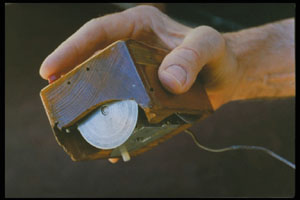
\includegraphics[width=0.3\linewidth]{figures/mouse.jpg}
	\caption{The first mouse}
\end{figure}

New and revolutionary ideas are required to create new peripherals that improve productivity, but are still intuitive and thus easy to learn to use. To get inspiration for improvement, one can look around and study already existing communication methods, for example the communication between humans. 

When two people are in a room and don't have a audio or visual limitation, they will probably communicate by speech. But there is much more going on than only producing and interpreting words. The intonation, speed and other small variations in the voice add a lot more information to the words. Also the facial expression and body language give more space for expression. Some people like to 'talk with their hands' while telling a story, something that adds more expression to the transmitted information.

\section{Sign Language}

A deaf person can't interpret spoken words, at least not by listening. He or she is highly depended on visual information. Sign languages have been created or invented to aid this visual communication. In these languages two elements have an important role, the face and the hands. These body parts give the most expressive power. The face because it is very good for expressing feelings and emotions, and the hands because they are very flexible and morphable. The hands are especially interesting because there are countless combinations of finger poses and orientations. 

Speech generation, speech recognition, facial expression recognition and sign language interpretation are all subject of extensive research at the moment.

Research has been done in automated sign language interpretation using computer vision\cite{Buehler2009}\cite{RichardBowden2004}. The problem with interpreting sign language is a very large vocabulary, segmentation of the different gestures and representing the gestures in a robust way.

\section{Goal and motivation}
\label{sec:goal}
The goal of this thesis is to describe the design, build and evaluation process of a system for hand pose recognition. The system needs to be fast and user friendly. Also the system should be able to run on current consumer hardware.

\begin{itemize}
	\item Real time performance (10+ fps)
	\item Normal consumer processing power
	\item Normal RGB camera (webcam)
	\item No gloves or skin mounted electromechanical sensors
	\item No calibration or initialization
	\item Minimal configuration/parameters
\end{itemize}
	

To realize these requirements some restrictions on the system's setting are required:
\begin{itemize}
	\item One person in the image
	\item Person is wearing clothing with long sleeves
	\item Good enough lightning conditions
	\item No skin like colors in the image.
\end{itemize}

The system can be used to aid HCI, but als add more feeling and detail, especially for real time interaction. Using hand poses for Computer aided music composing is interesting but challenging, since the realtime element plays an important role. Also, in a live performance setting, it is much more interesting to look at somebody using his body to interact with a machine than only click of a mouse.


\section{Solfege, The Curwen Hand symbols}

Any set of hand poses would do for this system, as long as the individual poses don't look to similar. But since the idea is to translate the interpreted hand poses into sound, it would be interesting to use a set of poses that has a already existing relationship to sound.

In Medieval music, the Guidonian hand was a mnemonic device used to assist singers in learning to sight sing. The idea of the Guidonian hand is that each portion of one hand represents a specific note within the hexachord system, which spans nearly three octaves. The other hand is used to point to the correct hand portion. \autoref{fig:guidonian} shows a hands with the tonal positions.

\begin{figure}[htbp]
	\center{}
	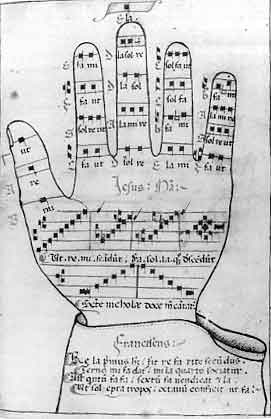
\includegraphics[width=0.3\linewidth]{figures/guidonian_hand.jpg}
	\label{fig:guidonian}
	\caption{Guidonian Hand}
\end{figure}

Despite this system has a large set of symbols - 22 to be exact - this system is not usable since the individual poses are very much alike. Discriminating between the different poses will probably be problematic.

A more recent method using hand poses in relation to music are the Curwen solfege hand signs\cite{choksy1999}. This method was introduced in the 19th century by John Curwen, who also is the founder of the famous tonic sol-fa. The tonic sol-fa is better known as \emph{'do re mi fa sol la ti'}.

\begin{figure}[htbp]
	\center{}
	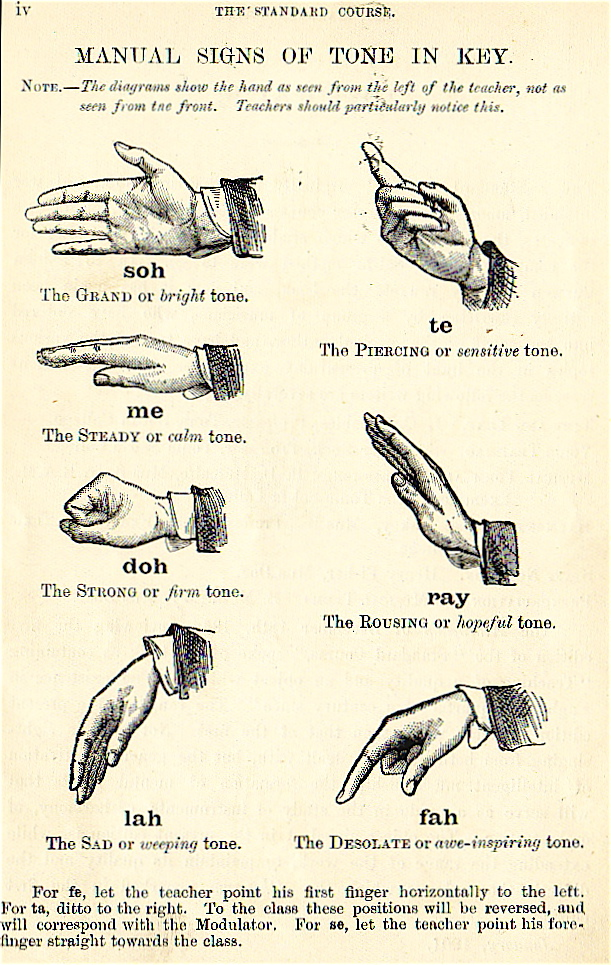
\includegraphics[width=0.6\linewidth]{figures/curwen.jpg}
	\label{fig:curwen}
	\caption{Depiction of Curwen's Solfege hand signs from 1904. This version includes the tonal tendencies and interesting titles for each tone.}
\end{figure}

\autoref{fig:curwen} is a scan from a teaching book from 1904 where the 6 tonal hand poses are shown. These 6 poses correspond to the 6 notes in the musical major scale. These hand poses are much more suitable for our system, since the individual hand symbols are distinct. Also the hand poses can be easily performed by both hands individually next to the body or in front of the body. \autoref{fig:curwennotes} shows the same hand symbols with the correspronding musical tones.

\begin{figure}[htbp]
	\center{}
	\subfloat{
		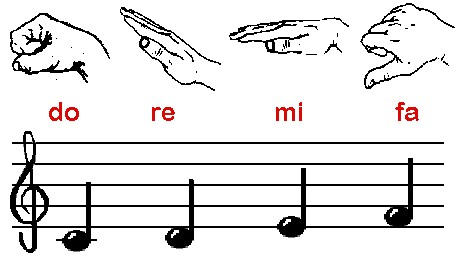
\includegraphics[width=0.45\linewidth]{figures/doremifa.jpg}
	}
	\hspace{0.03\linewidth}
	\subfloat{
		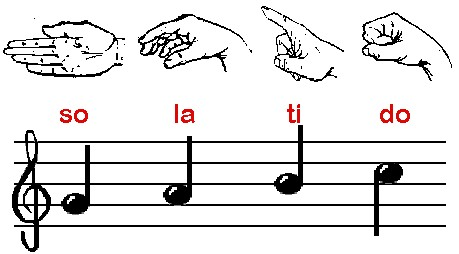
\includegraphics[width=0.45\linewidth]{figures/solatido.jpg}
	}
	\caption{The curwen hand symbols and the corresponding musical notes}
	\label{fig:curwennotes}
\end{figure}




\section{Related Work}
At the moment of writing this thesis Microsoft is finishing the development of a new commercial product called 'Kinect'. Kinect is claimed to provide full-body 3D motion capture. To accomplish this, Kinect uses a range camera, which interprets 3D scene information from a continuously-projected infrared pattern. For this setting a infrared projector and a range camera is required.

non-intrusive

\begin{figure}[htbp]
	\center{}
	\label{fig:kinect}
	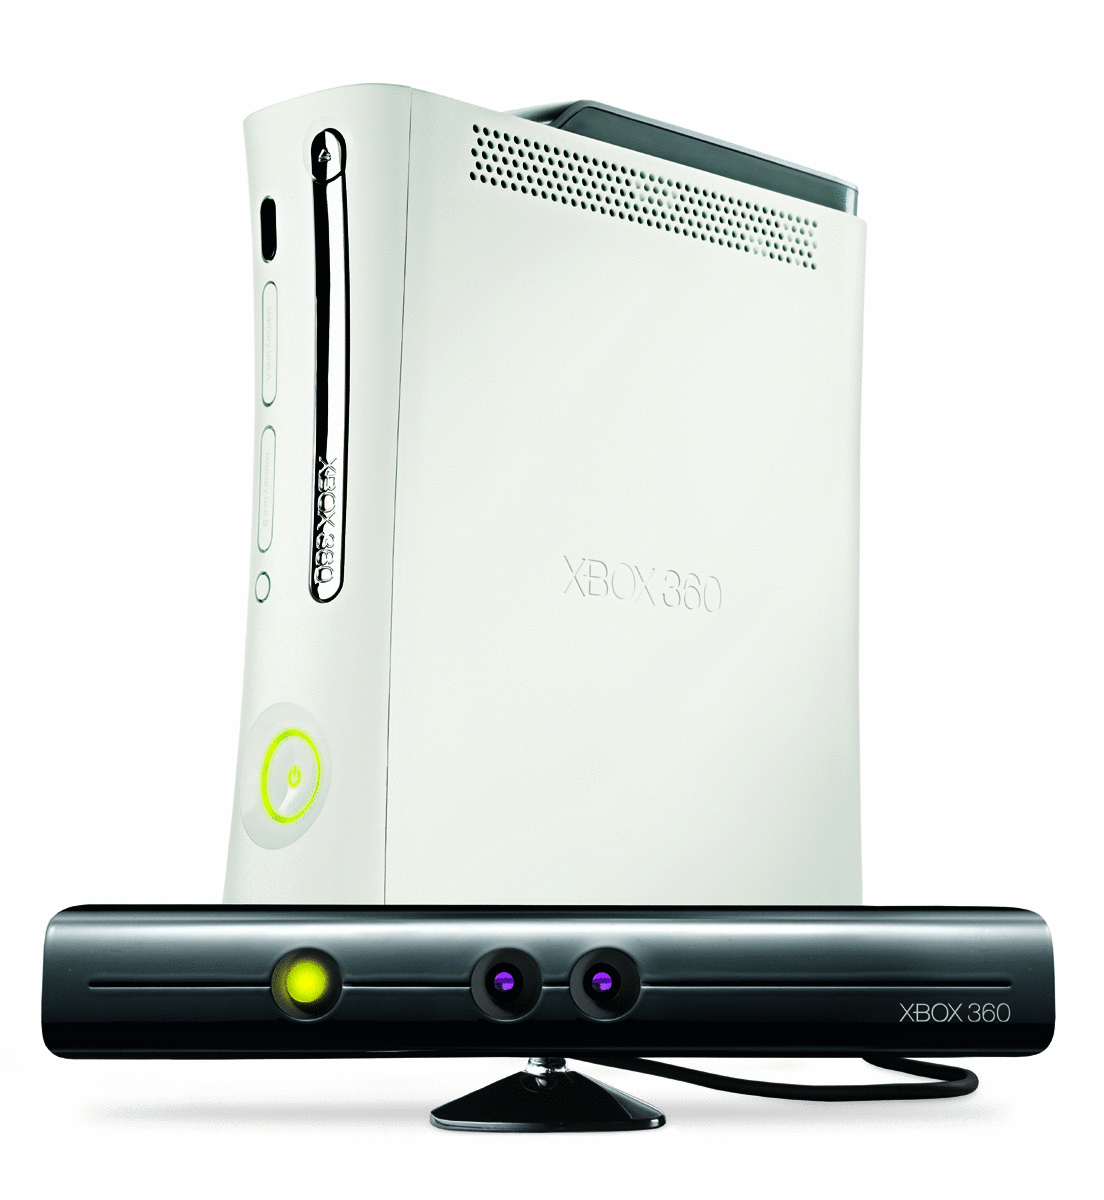
\includegraphics[width=0.3\linewidth]{figures/wave.jpg}
	\caption{Microsoft Kinect}
\end{figure}


An other interesting development is \cite{Wang2009} where a colored glove is used to perform full 3d hand pose estimation.

\begin{figure}[htbp]
	\center{}
	\label{fig:wang2009}
	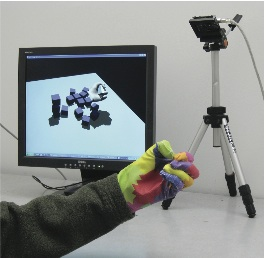
\includegraphics[width=0.3\linewidth]{figures/wang2009.jpg}
	\caption{3d hand pose estimation using a colored glove}
\end{figure}

An interesting overview paper is \cite{Erol2007}, which reviews the current state, possibilities and limitations of computer vision based hand pose and gesture recognition.


Similar research has been done \cite{Wang2007}. Here SIFT features are used to discriminate 3 different hand symbols. A performance of 95.6\% is claimed using a the 'sharing feature concept'.





others:

A PhD thesis exploring the hand as a input device: \cite{Sturman1992}

A very old paper using hand motion for segmentation: \cite{Cui1996}

Color based tracking a face for computer input \cite{Bradski1998}

Old paper using shadows to estimate 3d hand pose \cite{Segen1999}





%!TEX root = thesis.tex

\chapter{Body Part Detection}
\label{ch:bodyparts}

To perform hand pose estimation of a person in a image, hands need to be localized in the image first. Hands are very changeable - they can have very different appearances and different orientations. Also hand size and shape but also skin color can be very different per person. This makes the localization a very difficult task. 

One way to localize the hands is by searching for skin like colors in an image given that this color profile is known. A generic skin color model based on average skin color has been constructed for this purpose\cite{Jones1999}. The problem with this method is that it fails when the skin color isn't 'pure', for example when it is colored by a light source. but this method is sensitive for error when the image is colored by a light source. Also, since the profile is very generic, it contains colors for many different skin colors. This introduces more false positives.

It would be much better to have a method for obtaining the skin color of a person in a image from that image itself. This can be done by extracting the skin model from the face, which is much easier to detect.

This chapter will first describe how this skin model is created, followed by how this skin model is used to find the skin pixels in the image. These found skin pixels are clustered and labeled as left hand, right hand and head. How the positions of these labeled body parts are stabilized is also explained and is followed by how self occlusion can be handled.

\section{Building a skin model}
\label{sec:skinmodel}

\subsection*{Face localization}

\begin{figure}
  \center{}
    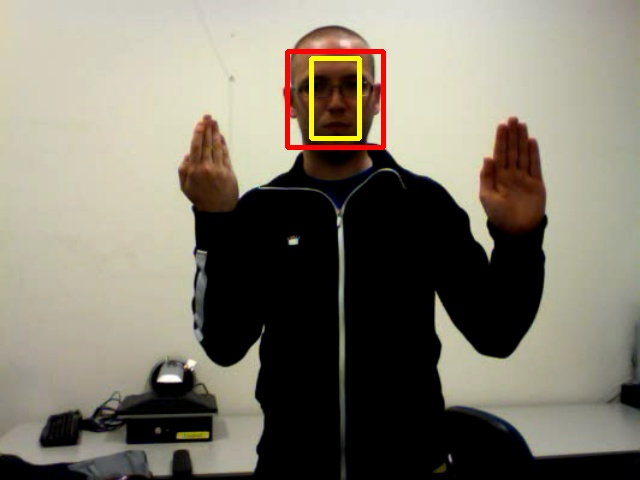
\includegraphics[width=0.6\textwidth]{figures/pipeline/detected.jpg}
  \caption{Face detection}
  \label{fig:face_detection}
\end{figure}


Finding faces in a image is a rather well solved problem. Faces are easy to detect, since it has easy to detect features like eyes, eyebrows, a mouth and a nose. When comparing different faces, these features are - with a small variation - on the same distance and orientation. Also people don't tilt their head often, or not more than a couple degrees. Face detection can be done in a fast and robust way using a haar classifier, a boosted rejection cascade that is trained with Haar\-like wavelet\cite{Lienhart2002}. This is a method for detecting faces that doesn't rely on color information. The classifier is run over the image on different scales, and positions with a score above a certain threshold are classified as face position.

The face detection is one of the most expensive operations used in this thesis. Since usually a face doesn't move fast in a vide stream, a number of frames can be skipped which will free more computational time for other operations.

Using a haar classifier to search for a face and obtain a skin color profile has been done before with the lab color space \cite{Stenger2006}, but in this case the HSV color space is used.

\subsection*{Color space conversion}
Usually, pixel values of a image are stored in the Red, Green Blue (RGB) color space where colors are represented with combinations of these primary colors. The RGB representation of colors is not suitable for modeling skin color. The RGB color space represents not only color, but also luminance which is not a reliable measure for segmenting skin pixels\cite{Cai1999}.

When a subject is lighted by a light source with uniform hue distribution, the light doesn't change the hue or saturation of the subject. The only thing that will change is the luminance, which is changing because of the light source's intensity, distance or (self casted) shadow. Since we want to extract hand pixels independent of the illumination intensity, we can ignore this channel and only use the hue and saturation.

The luminance can be removed from the color space by transforming the color model to a chromatic color space. There are multiple chromatic color spaces, for example LAB, HSV and normalized. A small experiment with these color spaces have shown that no significant improvements can be gained with a specific color space, so the HSV color space is used in the rest of this paper.


\begin{figure}[htbp]
  \centering
\subfloat[HSV color space]{
	\label{fig:hsv}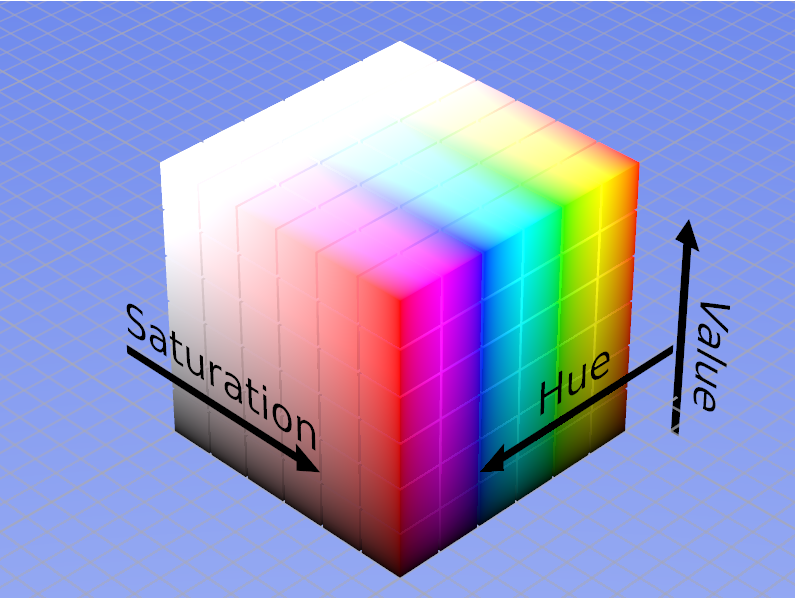
\includegraphics[width=0.45\linewidth]{figures/hsv2.png}
}
\hspace{0.01\linewidth}
\subfloat[RGB color space]{
	\label{fig:rgb}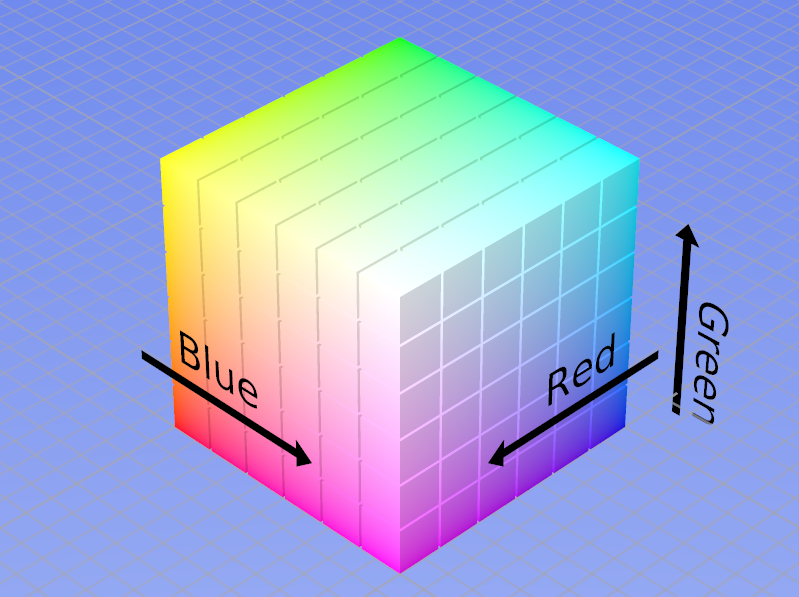
\includegraphics[width=0.45\linewidth]{figures/rgb.png}
}
  \caption{The RGB and HSV color space}
  \label{fig:colorspaces}
\end{figure}

HSV stands for hue (color), saturation (how concentrated the color is) and value (brightness). The brightness is changed by the illumination, so we will discard this channel

In practice a light source never has a uniform distribution and \emph{will} change the color of the subject. Since we build a color model from the image itself, all skin pixels will change in the same way. 

The RGB color space is transformed into the HSV color space using the following equations:
\begin{eqnarray*}
  V & \leftarrow & \max(R,G,B) \\
  S & \leftarrow & \left\{
  \begin{array}{l l}
    \frac{V-\min(R, G, B)}{V} & \quad \text{if $V \neq 0$} \\
    0 						  & \quad \text{otherwise} \\
  \end{array} \right.\\
  H & \leftarrow & \left\{
  \begin{array}{l l}
    \frac{60(G - B)}{S}     & \quad \text{if $V = R$} \\
    \frac{120 + 60(B-R)}{S} & \quad \text{if $V = G$} \\
    \frac{240 + 60(R-G)}{S} & \quad \text{if V = B} \\
  \end{array} \right.\\
\end{eqnarray*}

The input 3 channel RGB image is transformed into a 3 channel HSV image, after which the value channel is discarded. Using the detected face region of the hue and saturation channel a histogram can be constructed which will represent a statistical skin model.

\begin{figure}[htbp]
  \centering
\subfloat[hue channel]{\label{fig:hue}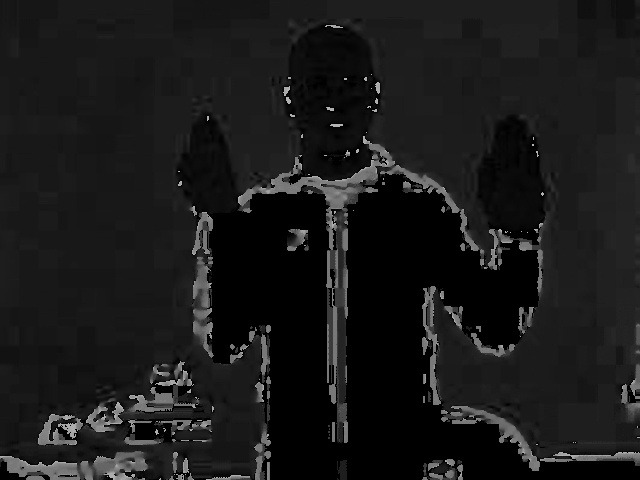
\includegraphics[width=0.3\linewidth]{figures/pipeline/hue.jpg}}
\hspace{0.03\linewidth}
\subfloat[saturation channel]{\label{fig:saturation}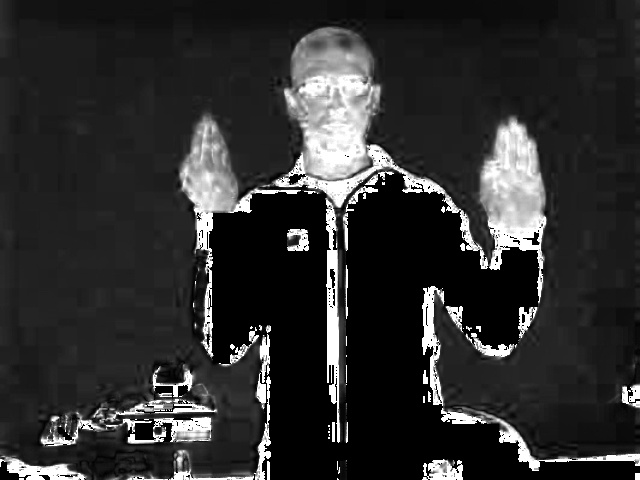
\includegraphics[width=0.3\linewidth]{figures/pipeline/saturation.jpg}}
\hspace{0.03\linewidth}
\subfloat[value channel]{\label{fig:value}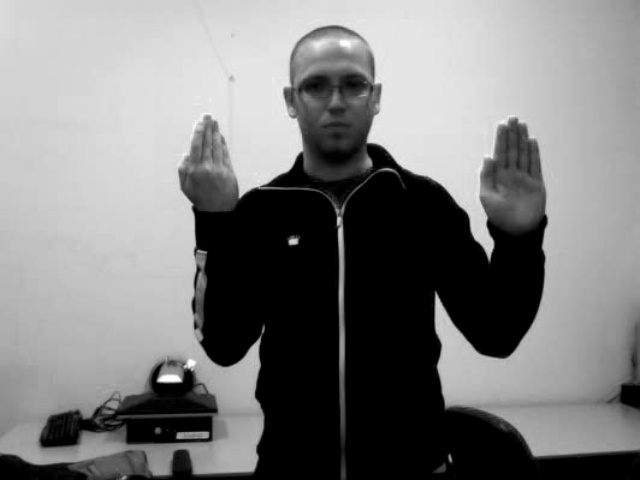
\includegraphics[width=0.3\linewidth]{figures/pipeline/value.jpg}}
  \caption{The HSV channels}
  \label{fig:hsvchannels}
\end{figure}





\subsection*{Statistical skin color model}

\begin{figure}[htbp]
    \center{}
    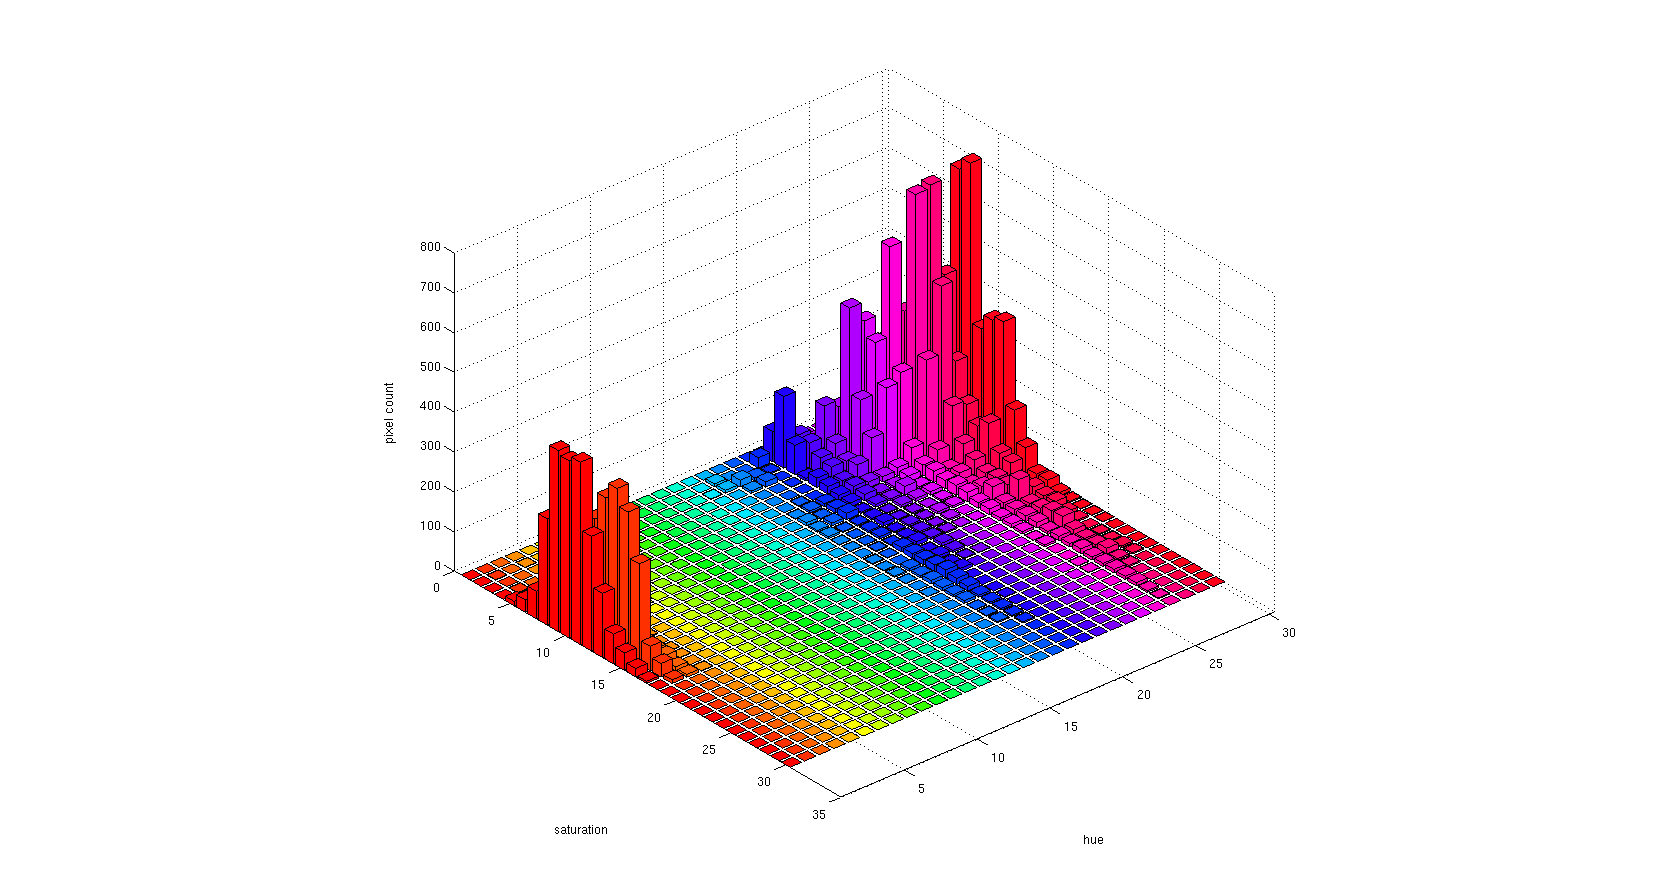
\includegraphics[width=1\textwidth]{figures/pipeline/histogram.png}
	\caption{A histogram of face pixels}
	\label{fig:histogram}
\end{figure}

There are multiple ways of constructing a statistical skin color model. The most conventional ways are a (mixture of) gausian(s) or a histogram. 

The skin color model is represented in a 2 dimensional histogram, where the first dimension is Hue and the second is Saturation. The histogram is filled with the values from the detected face region. After, the histogram is normalized - all values are divided by the sum of all bins. This makes the histogram independent of the original image size, and each histogram bin value represents a 'skin probablility'. \autoref{fig:histogram} is a histogram of colors of a caucasian.

Manual experiments show that tweaking the number of bins doesn't have much effect, as long as the number of bins is not too high or not to low. Since for the storage of the values a 8 bit integer is used, a number of bins higher than 256 doesn't make sense. In all experiments mentioned in this paper a number of bins of 30 is used for both the hue and saturation.

\subsection*{Back projection}

\begin{figure}[htbp]
    \center{}
    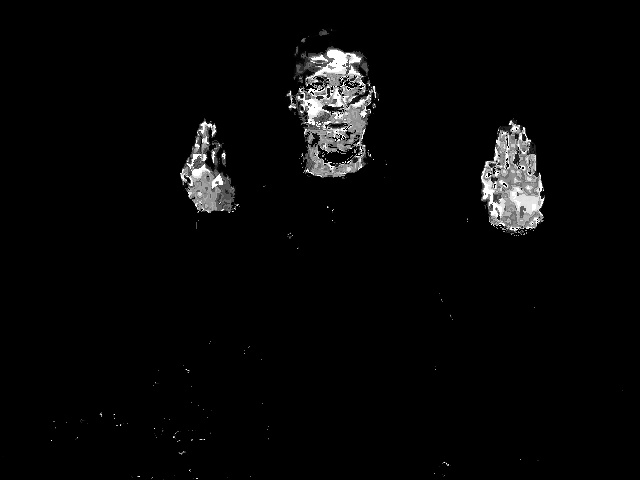
\includegraphics[width=0.5\textwidth]{figures/pipeline/backproject.jpg}
 	\caption{Backprojection}
	\label{fig:backproject}
\end{figure}


A back projection is the combination of an image and a histogram. The result is a new single channel image. All pixels in the input image are iterated and the corresponding bins are looked up in the histogram. The pixel in the same position in the new image is replaced with the value from the histogram. If the histogram is a skin color histogram, the resulting image will have high values for pixels that are skin-like pixels, and low values for other pixels. The result of the process can be seen in \autoref{fig:backproject}. Since the probabilities are very low the contrast of this image is enhanced so the maximum pixel value becomes pure white.


\subsection*{smoothing}
The back projection can be quite noisy, this is caused by the rounding in the in the histogram, but also by noise introduced by the camera. Thresholding this image will result in skin pixel groups with rough edges and a lot of holes, see \autoref{fig:threshold_noblur}. The noise can be reduced by smoothing the image. This way, the pixel value is replaced by the old value weighted with the surrounding pixel values. Using a gaussian kernel with a large size gives a good result, see \autoref{fig:blurred}.

\begin{figure}[htbp]
    \center{}
    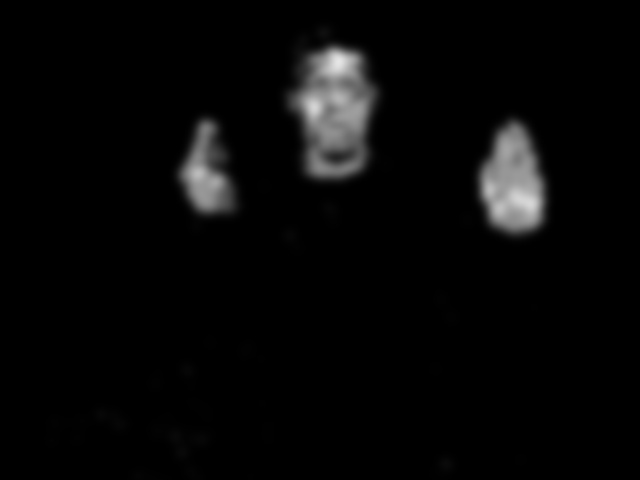
\includegraphics[width=0.5\textwidth]{figures/pipeline/blurred.jpg}
	\caption{Blurred image}
	\label{fig:blurred}
\end{figure}


\subsection*{Threshold}

\begin{figure}[htbp]
    \center{}
 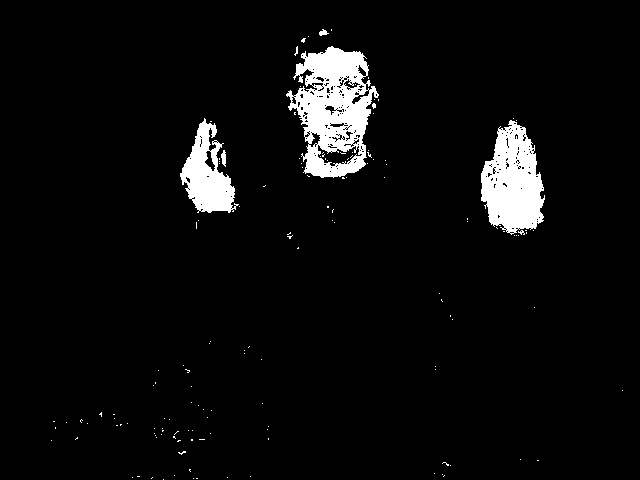
\includegraphics[width=0.5\textwidth]{figures/pipeline/thresholded_noblur.jpg}
	\caption{Thresholded image without blur preprocessing}
	\label{fig:threshold_noblur}
\end{figure}

\begin{figure}[htbp]
    \center{}
    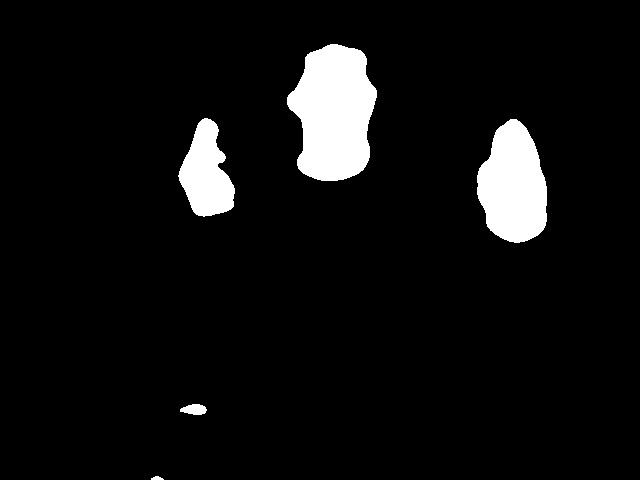
\includegraphics[width=0.5\textwidth]{figures/pipeline/thresholded.jpg}
	\caption{Thresholded image}
	\label{fig:threshold}
\end{figure}


To segments pixels from non-skin pixels we need to define a way of doing this automatically. The easiest way to accomplish this is by defining a threshold. All pixel values below a certain threshold are replaced with false or 0, all above this threshold will be replaced with true or 1. This results in a binary image with labels for (non) skin pixels. This introduces one parameter - the 
threshold for going from the probabilistic domain to the binary domain.

A alternative method of going from the probabilistic domain to the binary domain is adaptive thresholding. here the threshold is determined per pixel by the values of surrounding pixels. This method has one parameter; the neighborhood blocksize used to determine the threshold.


\subsection*{morphological operations}

\begin{figure}[htbp]
    \center{}
    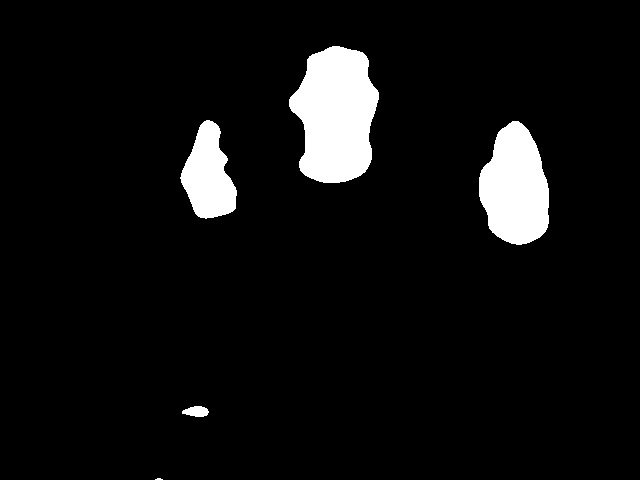
\includegraphics[width=0.5\textwidth]{figures/pipeline/closed.jpg}
	\caption{Morphologically closed}
	\label{fig:closed}
\end{figure}

An alternative to smoothing out rough edges and holes are (combinations of )morphological operations.  A morphologic closing operation of A by B is obtained by the dilation of A by B, followed by erosion of the resulting structure by B. The result of performing this operation is that small holes in the binary image are removed, and edges are smoothed as seen in \autoref{fig:closed}. The effect isn't really significant, since the gaussian smoothing already removes a lot of noise. 


\section{Object localization}

\subsection*{Pixel grouping, contour extraction}
To be able to say something useful about groups of pixels, one need to know which pixels belong together. This is done by clustering. In this case clustering is performed by grouping pixels together to touch horizontally and vertically. Each cluster of pixels is called a blob.

To handle the blobs in a time efficient way, it is good idea to extract the contours. This way interesting problems can be solved like if a certain pixel coordinate is inside a certain blob, the maximum or minimal horizontal or vertical position and hole removal.

Since it unusual to have holes in blobs that represent skin regions, these can be removed. This is done with the algorithm described in \cite{Suzuki1985}, where the contours of the blobs are extracted and all contours except the outer most contour are removed. This removes holes and islands in holes.

From the contours of the group a square region of interest is defined by calculating the outer borders of the group. This window is called the hand window from now on.

\subsection*{Blob labeling}

\begin{figure}[htbp]
    \center{}
    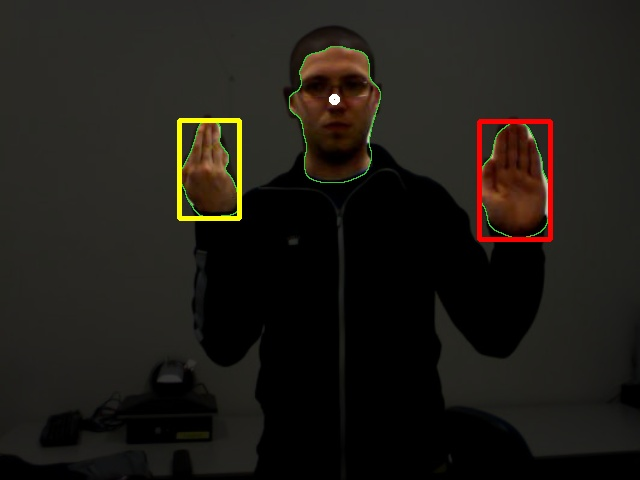
\includegraphics[width=0.5\textwidth]{figures/pipeline/contours.jpg}
	\caption{Labeled blobs}
	\label{fig:contours}
\end{figure}


Now we have blobs we need to know blob is what body part. In a optimal situation there are three blobs, two for the hands and one for the head. For one blob it is already known what body part it is - the face. In the face detection phase we found a face in the image, so the blob containing the center point of the detected phase is the face blob. Usually the left hand is on the left of the head and the right hand on the right side. If there are three blobs, and the face is the middle blob, we labeling is done. If not an other decision needs to be made. Often there are more or less blobs, because the background has skin-like color, a hand is difficult to detect or is occluded. Also the order of hands and head can change, a left hand doesn't necessarily need to appear on the left side of a head.

First the surface of each blob is calculated and then the blobs are sorted by size. The blob containing the head is removed from the list, since we already know this label. Also very small blobs are removed, because these are probably noise. The removal threshold surface is set to:

\begin{equation}
T = (\frac{h}{c})^2
\end{equation}

Where $h$ is the height of the movie frame and $c$ is a control constant. The equation can be interpreted as a filter for the minimal size in square pixels, relative to the hight of the movie frame. A value of $20$ for $c$ removes a lot of noise blobs, but still is small enough to leave most hand blobs intact.

Assuming the hands or the second biggest skin like objects in the image, the 2 or less biggest blobs are taken from the list and the rest is also discarded. If there is no biggest blob, the labeling is finished - there is only a head in the image. If there is one blob left, the left or right position relative to the head is the hand label. If there are 2 hands, there are 3 possible situations, 1 where the head is in the middle which is already described. If both hands are on the left of the head, the most outer left blob is labeled as left and the other as right. This is visa versa for right.

\begin{algorithm}
\caption{Blob labeling heuristics}
\label{blobheuristics}
\begin{algorithmic}
	\STATE head $=$ left $=$ right $=$ None
	\STATE faceCenter $=$ getFaceCenter()
	\STATE blobs $=$ getContours()
	\STATE limbs $=$ []
	
	\FOR{blob in blobs}
		\IF{blob.contains(faceCenter)}
			\STATE head $=$ blob
		\ELSE
			\STATE blobs.append(blob)
		\ENDIF
	\ENDFOR

	\STATE blobs $=$ sortBySize(blobs)
	\STATE blobs $=$ blobs[-2:]
	\STATE blobs $=$ sortByXPosition(blobs)

	\STATE $n = $ len(blobs)
	\IF{$n == 2$}
	    \STATE left $=$ blobs[0]
	    \STATE right $=$ blobs[1]
	\ELSE
		\IF{$n == 1$}
		    \IF{blobs[0].center[0] $<$ face\_center[0]}
		        \STATE left $=$ blobs[0]
		    \ELSE
		        \STATE right $=$ blobs[0]
			\ENDIF
		\ENDIF
	\ELSE
	    \STATE print("didn't find any limbs")
	\ENDIF
\end{algorithmic}
\end{algorithm}



\subsection*{Blob label stabilization}
A hand doesn't move very fast in an image - usually it will not move from the left side to the right side in one frame. If this is detected this is probably a measurement error caused by noise or pour labeling. In this case the history of previous positions of a blob can be incorporated. This can be done with a Kalman Filter. A Kalman Filter is a easy and fast way of smoothing out the current position with the previous positions. The result will be a more stable estimation of the hand position. A second advantage of the Kalman Filter is the ability to actually predict the position of the hand in the next frame. This can become useful when there is no new hand detected. The hand position can then be estimated with a different method.

For every hand a Kalman filter is initialized. The measurement that need to be smoothed is the hand window. The hand window has a x and y position and a width and hight. Each hand also has a speed in the x and y direction but we don't measure that - we let the kalman filter represent, calculate and use that internally. 

A hand window represented in a measurement vector as:

\[ m_k = \left(
\begin{array}{c}
	x_k \\ %measurement.x
	y_k \\ %measurement.y,
	w_k \\ %measurement.width
	h_k \\ %measurement.height
\end{array} \right)\]

Where $x_k$ is the horizontal position, $y_k$ is the vertical position, $w_k$ is the width and $h_k$ is the height of the hand window.

The Transition matrix is defined as follows:

\[ A = \left(
\begin{array}{cccccc}
	1 & 0 & 0 & 0 & 1 & 0 \\
	0 & 1 & 0 & 0 & 0 & 1 \\
	0 & 0 & 1 & 0 & 0 & 0 \\
	0 & 0 & 0 & 1 & 0 & 0 \\
	0 & 0 & 0 & 0 & 1 & 0 \\
	0 & 0 & 0 & 0 & 0 & 1 \\
\end{array} \right)\] 

This is just an identity matrix, except for the left ones on the right top in the matrix. These represent the combination of the current position and the internal state of the speed.

With these matrixes and a standard kalman filter the position and size of the hands can be predicted. The predicted values are used for an other hand localization method in case no hand is found en the next frame.

% setIdentity(kalman.measurementMatrix, Scalar(1));
% setIdentity(kalman.processNoiseCov, Scalar(1));
% setIdentity(kalman.measurementNoiseCov, Scalar(5));
% setIdentity(kalman.errorCovPost, Scalar(3));
% setIdentity(kalman.gain, Scalar(0e-15));
% randu(kalman.statePost, Scalar(1), Scalar(100));



% \paragraph{Update}
% The kalman filter is then updated:
% 
% Innovation or measurement residual 	
% $\tilde{\textbf{y}}_k = \textbf{z}_k - \textbf{H}_k\hat{\textbf{x}}_{k|k-1}$

% Innovation (or residual) covariance
% $\textbf{S}_k = \textbf{H}_k \textbf{P}_{k|k-1} \textbf{H}_k^\text{T} + % \textbf{R}_k$

% Optimal Kalman gain
% $\textbf{K}_k = \textbf{P}_{k|k-1}\textbf{H}_k^\text{T}\textbf{S}_k^{-1}$

% Updated (a posteriori) state estimate
% $\hat{\textbf{x}}_{k|k} = \hat{\textbf{x}}_{k|k-1} + % \textbf{K}_k\tilde{\textbf{y}}_k$

% Updated (a posteriori) estimate covariance
% $\textbf{P}_{k|k} = (I - \textbf{K}_k \textbf{H}_k) \textbf{P}_{k|k-1}$

% \paragraph{Prediction}
% And the values are predicted with:

% Predicted (a priori) state estimate 	
% $\hat{\textbf{x}}_{k|k-1} = \textbf{F}_{k}\hat{\textbf{x}}_{k-1|k-1} + % \textbf{B}_{k} \textbf{u}_{k}$

% Predicted (a priori) estimate covariance
% $\textbf{P}_{k|k-1} = \textbf{F}_{k} \textbf{P}_{k-1|k-1}
% \textbf{F}_{k}^{\text{T}} + \textbf{Q}_{k}$


\subsection*{Self occlusion by body parts}
When in a previous frame a hand was detected but in the current frame not any more three things can be the source. First of all the hand can be out of the image, or occluded by an obstacle. The second case is that the hand detection phase just fails and couldn't localize the body part. The third case is self occlusion, where the hand is very close or occluding the hand and the skin segmentation segements these two bodyparts as one. In this case template search is used to track the specific hand. A cut out image of the hand in the previous frame is used for this template search. Template search is a very simple and fast method, as long as the search area is small. A sliding window  with the same size as the cutout image is sliding over a small surrounding area of the location predicted by the kalman filter. The window with the lowest squared sum difference to the previous cutout image is set as the new location. If the original cutout is touching the border of the image or the squared sum difference is to high it is assumed the hand has left the image, and is flagged accordingly. This method works if the shape and size of the hand don't change too much.

\begin{figure}[htbp]
\begin{center}
\subfloat[detected hand]{\label{fig:template_good}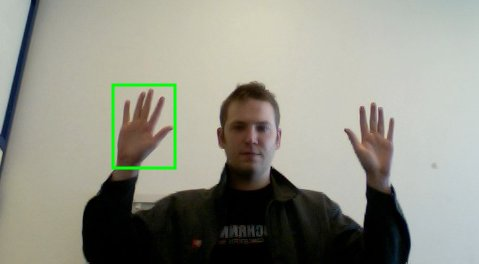
\includegraphics[width=0.45\linewidth]{figures/template/good.jpg}}
\hspace{0.03\linewidth}
\subfloat[result of template search]{\label{fig:template_occlusion}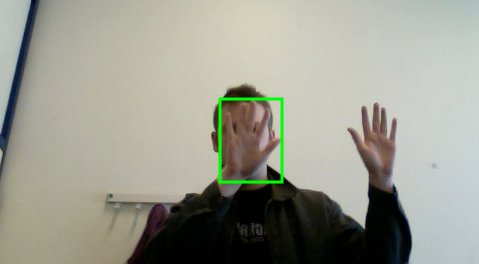
\includegraphics[width=0.45\linewidth]{figures/template/occlusion.jpg}}
\end{center}
\caption{Example of template search}
\label{fig:templatesearch}
\end{figure}

\autoref{fig:templatesearch} shows a test setting of a template search. In the left image The left hand was found using the skin model. In the second frame the hand cannot be found, because it is occluding the face and using the skin model approach the hand will be labeled as face. Using a template search the hand can still be tracked.


\section{Discussion}
This method is quite robust, but can fail if the conditions listed in \autoref{sec:goal} are not met. See \autoref{fig:fail} for an example of failed segmentation. This figure is a still from one of the movies in the dataset used in the experiments. The test subject has a skin color profile that is similar to parts of the background. Not much can be done to solve this problem, except the threshold can be manually adjusted. Still, this will introduce more false negatives and the segmentation will still be poor.

\begin{figure}[htbp]
\center{}
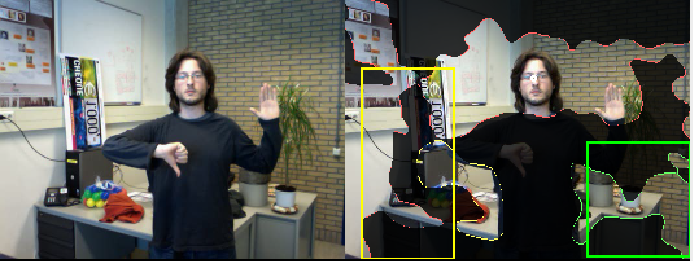
\includegraphics[width=0.8\linewidth]{figures/fail.png}
\caption{Example of failed segmentation}
\label{fig:fail}
\end{figure}








%!TEX root = thesis.tex

\chapter{Gesture recognition}
\label{ch:gestures}



\section{Feature extraction}

\subsection*{Segmentation - removing background}

\begin{figure}[htbp]
\begin{center}
\subfloat[Hand window]{
        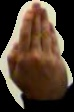
\includegraphics[width=0.2\linewidth]{figures/pipeline/lefthand.jpg}
        \label{fig:lefthandwindow}
}
\hspace{0.03\linewidth}
\subfloat[Hand cutout]{
        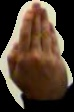
\includegraphics[width=0.2\linewidth]{figures/pipeline/lefthandcutout.jpg}
        \label{fig:lefthandcutout}
}
\hspace{0.03\linewidth}
\subfloat[Hand features]{
        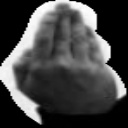
\includegraphics[width=0.2\linewidth]{figures/pipeline/lefthandhog.jpg}
        \label{fig:lefthandfeatures}
}
\end{center}
\end{figure}

A cutout of a hand from a image still contains some background pixels, because a hand will never fill a perfect square. These pixels are unwanted since they contain arbitrary values that introduce noise into our process. In section \ref{sec:skinmodel} a binary mask for skin pixels is constructed. The binary inversion of this mask can be used again to remove the background. The result of this procedure can be seen in figure \ref{fig:gijs5_cutout}. To decrease the possibility that mislabeled skin pixels are removed by this mask, a small morphological dilate operation will increase the size of the hand cutout, but this will also introduce more noisy (background) pixels.


\subsection*{Histogram of Oriented Gradients}
Histogram of oriented gradient (HOG) descriptors are feature descriptors used for object detection. It has been successfully applied and studied in human detection \cite{NavneetDalal2006}.  The HOG descriptors method is similar to that of edge orientation histograms, scale-invariant feature transform descriptors, and shape contexts, but differs in that it uses a dense grid of uniformly spaced cells and uses overlapping local contrast normalization for improved accuracy.

For the experiments described in chapter \ref{ch:experiments} the same parameters as in the \cite{watanabe2009} paper are used, except that the image is not resized to 64 by 128 pixels, but 128 by 128 pixels.

hand detection with SIFT\cite{Wang}

\section{Classification}

\subsection*{Classifier}
Two classifiers where evaluation during the experiments, K-Nearest Neighbors (KNN) and Support Vector Machines (SVM). For the experiments with KNN different values for $k$ where evaluated. The experiments with SVM where more profound, different kernels and parameters where evaluated. The evaluated kernels are the Radial Basis Function (RBF) and a precomputed kernel using the $\chi^2$ method on the train set. For the RBF kernel 2 parameters are important, the cost $c$ and $\gamma$. The optimal values of these variables for these experiments where found with a brute force grid search on a small cluster.

Also Principal Component Analysis (PCA) was performed on the dataset to reduce the dimensionality. The impact on the classifiers has been measured and is presented together with all other experiments in chapter \ref{ch:experiments}.

\subsection*{The stabilizer}
Since the frames following each other have a spatio-temporal relationship there is a relationship between the labels given by the classifier. Because of noise, misclassification can happen. These false matches can be filtered out by smoothing the labels on a time scale.

This smoothing is done with a simple self invented method called 'the stabilizer'. 

The stabilizer is initialized with $n$ numbers of bins which is equal to the number of labels. There are 2 parameters, $n_{max}$ and $n_{threshold}$.

For every new label that is given by the classifier all bins are decremented with 1, except for the bin with the currently classified label which is incremented. A bin is incremented until it reaches it maximum value. When at any moment one of the bins value rises above the threshold, the stabilizer will output the label of that bin, as if it was the classifier itself. The result is a more stable and smoothed stream of labels, where single noisy labels are filtered out. For a sequence of frames with a correctly detected pose there is a delay between the first frame and the stabilizer will output the correct label, this delay is controlled by $n_{threshold}$ which is measured in frame count. A higher value will reduce more noise, but will give a bigger delay. There is also a delay after a sequence which is controlled by $n_{max}$. With a framerate of $25$ frames a second, $n_{max} = 15$ and $n_{threshold} = 10$ give good results reducing noise and still being very responsive. 

\subsection*{Training phase}
recording video, manual labeling, extracting HOG features, training classifier

\section{Discussion}


%!TEX root = thesis.tex

\chapter{Experiments}
\label{ch:experiments}


\section{The dataset}
A dataset was constructed to perform the experiments where people perform the Curwen hand poses in different settings. Usually the 12 Curwen solfege hand symbols are performed in front of the torso. To increase the number of hand poses to be recognized and increase the usability, all 12 Curwen are also performed mirrored next to the body of the recorded subject, see \autoref{fig:torso}. Additionally four extra hand symbols have been added that are not part of the Curwen sequence. These last four symbols are performed next to the head. This results in a total of 28 hand poses.

\begin{figure}[htbp]
  \centering
	\subfloat[in front of torso]{
		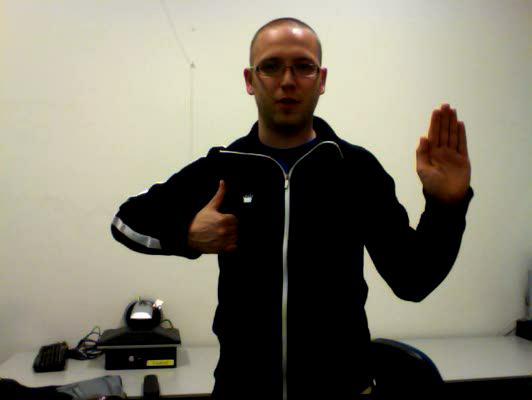
\includegraphics[width=0.4\linewidth]{figures/gijs5/13.png}
	}
\hspace{0.03\linewidth}
	\subfloat[next of torso]{
		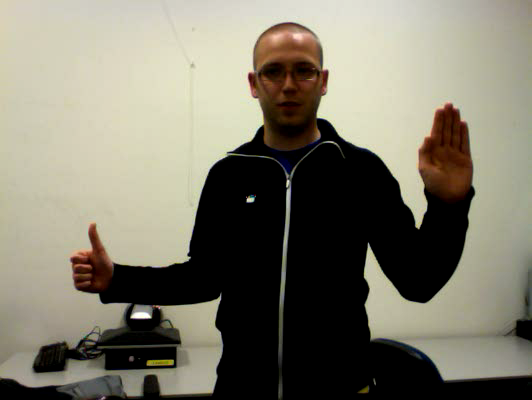
\includegraphics[width=0.4\linewidth]{figures/gijs5/1.png}
	}
  \caption{The Curwen hand poses}
  \label{fig:torso}
\end{figure}


In total there are 74 movies containing 20 different people performing the complete sequence of 28 hand symbols. At first people were recorded performing the complete sequence 5 times, but this was taking too much time, and people became impatient, after we switched to 3 movies per person. For each pose in each movie a frame was manually labeled where the person was performing the pose correctly.  The movies where recorded with  a resolution of 532x400 and a frame rate of 10. The test subjects were recorded while looking at a computer screen and asked to mimic the examples as in \autoref{fig:hands}. 12 test subjects where recorded with a simple (almost empty and smooth) background (\autoref{fig:simplebackground}), 3 where recorded with a complex background (\autoref{fig:complexbackground}) and 6 where recorded with the same complex background but also with a poster with skin like colors.

The nationality of the test subjects is diverse. Half of the set is Dutch and two are from South-East Asia. The rest is from eastern and southern Europe. (KLOPT DIT?)

\begin{figure}[htbp]
\center{}
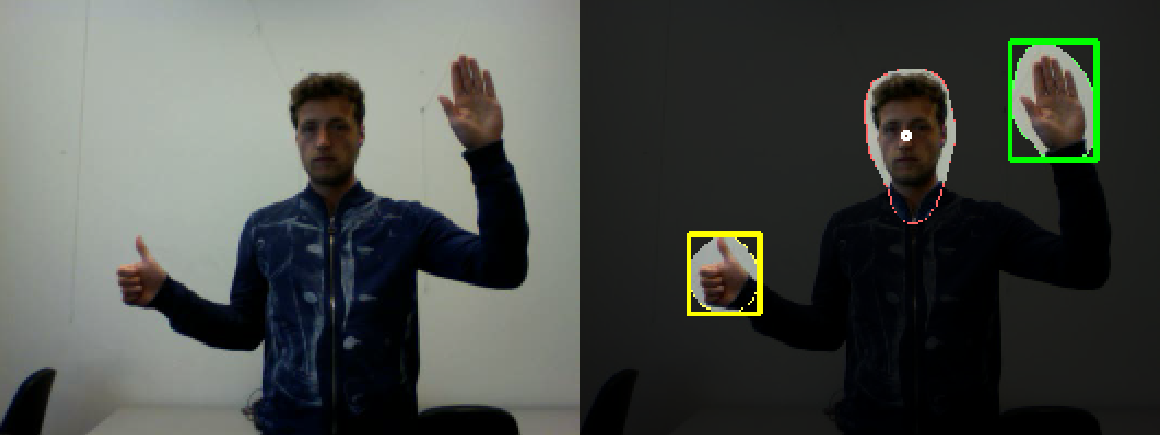
\includegraphics[width=0.8\linewidth]{figures/simple.png}
\caption{Still of movie ivo5 with simple background}
\label{fig:simplebackground}
\end{figure}

\begin{figure}[htbp]
\center{}
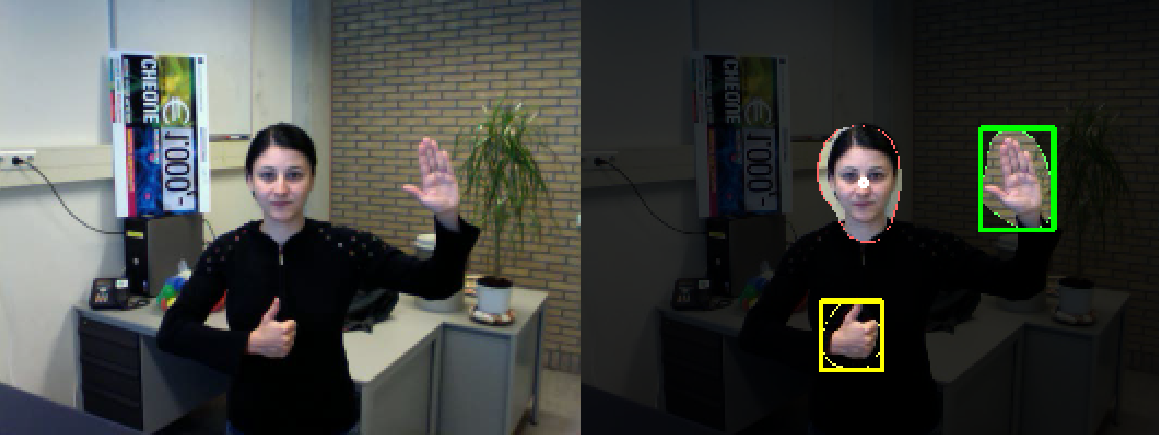
\includegraphics[width=0.8\linewidth]{figures/complex.png}
\caption{Still of movie gosia3 with complex background}
\label{fig:complexbackground}
\end{figure}

\begin{figure}[htbp]
\center{}
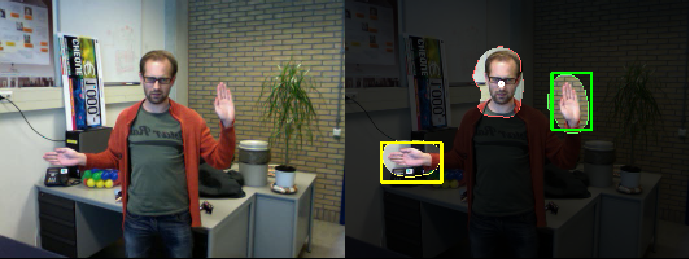
\includegraphics[width=0.8\linewidth]{figures/complexposter.png}
\caption{Still of movie sil1 with complex background with skin like poster}
\label{fig:complexposterbackground}
\end{figure}


\begin{table}
\centering
\begin{tabular}{llll}
\hline\hline
	Test Subject & Movies & Background &\\
\hline
	Anne     & 5 & Simple & \\
	Arjan    & 5 & Simple & \\
	Gijs     & 5 & Simple & \\
	Ivo      & 5 & Simple & \\
	Jasper 1 & 5 & Simple & \\
	Peter    & 5 & Simple & \\
	Hanne    & 5 & Simple & \\
	Jasper 2 & 3 & Simple & \\
	Ork      & 3 & Simple & \\
	Roberto  & 3 & Simple & \\
	Xirong   & 3 & Simple & \\
	Gosia    & 3 & Complex & \\
	Hamdi    & 3 & Complex & \\
	Michael  & 3 & Complex & \\
	Sil      & 3 & Complex + poster & \\
	Victoria & 3 & Complex + poster & \\
	Bas      & 3 & Complex + poster & \\
	Koen     & 3 & Complex + poster & \\
	Chu      & 3 & Complex + poster & \\
	Stratis  & 3 & Complex + poster & \\
\hline
\end{tabular}
\caption{Dataset details}
\end{table}

\section{Evaluation}

\subsection{part I - evaluating classifiers}
In this section different classifier with different parameters are evaluated with subsets of the dataset.

\subsubsection{Method}
All hand windows for each symbol in each movie are extracted and the features are extracted and stored. This data in then imported in Matlab, where the experiments are performed. For the SVM classifier the libsvm\footnote{http://www.csie.ntu.edu.tw/~cjlin/libsvm/} package is used. To perform PCA the prtools\footnote{http://www.prtools.org/} package is used. For nearest neighbors the KNN implementation in the biolearning package of matlab itself is used. The evaluation of the classifiers is split in three runs per classifier:

\paragraph{K-fold per movie using simple dataset only}
Only the movies with a simple background are used. For each run one movie is used for testing and all other movies are used for training. For each recorded person in the test set there are also 2 or 4 recordings of him or her used in the train set. This setting mimics the real life situation where the system is pre-trained with other people \emph{and} the user, with a simple background.

\paragraph{K-fold per person}
All movies or used, but per person the movies are used for testing and all other movies for training. Both complex and simple backgrounds are used. This setting mimics the real life situation where the system is pre-trained with only other people than the user of the system, and the background isn't necessarily simple. 

\paragraph{Simple as train set, complex as test set}
The classifier is trained with all movies with the simple background, and as a test set the movies with the complex background are used. This mimics the real life situation where the training is with recordings in optimal conditions, but the system is used in a complex environment like a living room. Also the system is not trained by the user.


\subsubsection{Test setting}
For the number of neighbors for K-NN a small number of tests where run, and a value between 3 and 10 for N yielded similar performance. Since a lower number of $k$ can give better performance $k=3$ was used for all experiments.

When PCA was performed on the dataset the smallest eigenvectors where removed so 95\% of the original variance was remaining. On the simple dataset reduce the dimensions from 3780 to 594 dimensions. For the complex set combined with the simple set the dimensionality is reduced to 688 dimensions, for complex only 283 and for the complete dataset 749.

For SVM two kernels are evaluated, RBF and $\chi^2$. The $c$ for both kernels and $\gamma$ for RBF values where found by an extensive grid search on the 'per person' test set with only the simple movies performed on a small cluster in the ranges $2^{-3}$ to $2^{15}$ for $c$ and $2^{-15}$ and $2^3$ for $\gamma$. The most optimal values for $\gamma$ is 0.03125. With this $\gamma$ changing the value for $c$ didn't have much effect on the performance, so a value of 64 was taken.

For calculating the HOG features the same parameters as \citep{watanabe2009} are used, except that the image is not resized to 64 by 128 pixels, but 128 by 128 pixels.

To be able to compare the HOG and SURF, the SURF descriptor is configured to work with a fixed set of interest points set up as a dense grid - the same set used for HOG. This results in a 13440 dimensional feature vector. Also using the interest point detection is a expensive operation, calculating this on a small image takes about 500 ms which makes it unusable for real-time operation.

\autoref{fig:lefthandfeatures} is an example of a image used for calculating HOG features.


The Curwen hand symbols that are closely related in a musical scale way are quite similar, for example 'Re' and 'Ri' (\autoref{fig:reri}). It is expected that a lot of misclassifications will be caused by this similarity. To investigate the impact, 2 different scores are calculated, one for the major scale and one for the full scale. The full scale threats every class as a single class, for the major scale the notes in the major scale and their corresponding similar notes are joined into one class. \emph{Do} is combined with \emph{Di}, \emph{Re} with \emph{Ri}, \emph{Fa} with \emph{Fi}, \emph{Sol} with \emph{Si} and \emph{La} with \emph{Li}.


\begin{figure}[htbp]
  \centering
\subfloat[Re]{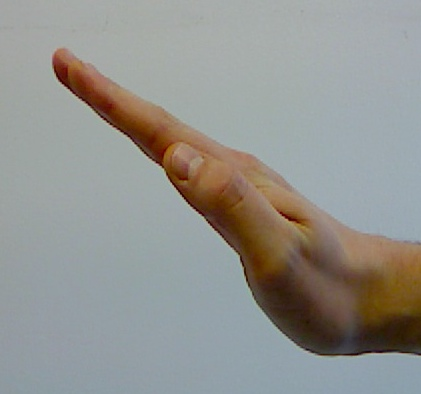
\includegraphics[width=0.2\linewidth,height=0.15\linewidth]{figures/examples/2.jpg}}
\hspace{0.03\linewidth}
\subfloat[Ri]{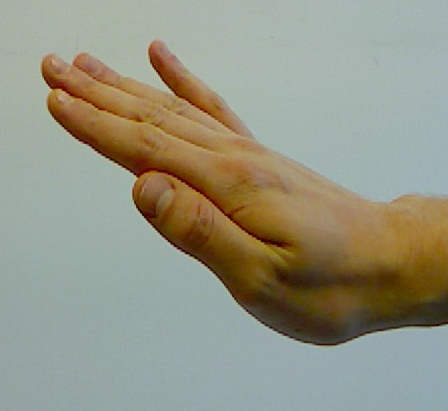
\includegraphics[width=0.2\linewidth,height=0.15\linewidth]{figures/examples/3.jpg}}
  \caption{Hand poses for \emph{Re1} and \emph{Ri1}}
  \label{fig:reri}
\end{figure}


\subsubsection{Results}
See \autoref{tab:perfilm}, \autoref{tab:perperson} and \autoref{tab:perset} for all the results, $f$ is the number of features. In all cases SVM performs better than KNN. The SURF features perform very bad compared to HOG. The $x^2$ distance kernel performs slightly better than the RBF kernel.  PCA improves performance when using a SVM classifier, but degrades the performance with KNN. 

\autoref{fig:confusion} is the confusion matrix of the best results from \autoref{tab:perfilm}, a SVM classifier with a precomputed kernel using the $\chi^2$ distance and HOG features. Most notable is the poor performance for the \emph{fi1} hand pose, see \autoref{fig:fi1}. This is probably due to the lack of skin surface and unique features. On the opposite \emph{sol1, do2, fa2, ti2, I, II, III }and \emph{IV}, perform near perfect. These hand poses expose a lot of surface and features. (MISSCHIEN PLAATJES HIER NOG EEN KEER)

\begin{figure}[htbp]
  \centering
  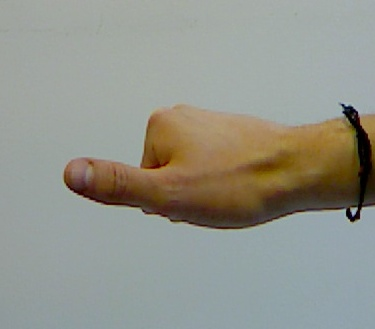
\includegraphics[width=0.2\linewidth]{figures/examples/6.jpg}
  \caption{Hand pose for \emph{fi1}}
  \label{fig:fi1}
\end{figure}


\begin{table}
\centering
\begin{tabular}{llrr}
\hline\hline
Classifier 		& PCA		&  	Full scale	& Major scale	\\
\hline
KNN3 		&	no	&  	84.27\%		& 90.21\%		\\
KNN3	 	&	yes	& 	83.67\%		& 89.70\%		\\
SVM RBF ($c=1$ $\gamma=\frac{1}{|f|}$)	&	yes	& 	76.78\%	& 84.38\%	\\
SVM RBF ($c=2^6$ $\gamma=2^{-5}$)		&	no	&	86.02\%	& 90.88\% \\
SVM RBF ($c=2^6$ $\gamma=2^{-5}$)		&	yes	& 	86.85\% & \textbf{91.85\%} \\
SVM $\chi^2$ &	no	&	\textbf{87.92\%}		& 91.58\% \\
SVM $\chi^2$ &	yes	&	TODO		& TODO \\
\hline
\end{tabular}
\caption{k-fold per film using simple dataset only,}
\label{tab:perfilm}
\end{table}


\begin{table}
\centering
\begin{tabular}{lllrr}
\hline\hline
Dataset & Classifier & PCA	& Full scale	& Major scale \\
\hline
simple	& KNN3	&	no	& 72.93\%, & 82.63\% \\
simple	& SVM RBF ($c=2^6$ $\gamma=2^{-5}$) &	yes	& \textbf{79.71\%} & \textbf{86.70\%}	\\
\hline
full 	& KNN3 &	no	& 66.98\% & 76.32\%	\\
full 	& KNN3 &	yes	& 65.31\% & 76.00\%	\\
full 	& SVM RBF ($c=1$ $\gamma=\frac{1}{|f|}$) & yes	& 64.05\% & 74.42\%	\\
full 	& SVM RBF ($c=2^6$ $\gamma=2^{-5}$)	     & yes	& \textbf{73.38\%} & \textbf{81.44\%}	\\
full 	& SVM $\chi^2$ &	no	&  71.83\% &80.07\% \\
full 	& SVM $\chi^2$ &	yes	&  TODO & TODO \\
\hline
\end{tabular}
\caption{k-fold per person}
\label{tab:perperson}
\end{table}


\begin{table}
\centering
\begin{tabular}{lllcc}
\hline\hline
Descriptors & Classifier 		& pca		&  	Full scale	&	Major scale	\\
\hline
Hog & KNN3				& no	&	58.57\% 	&	72.78\%	\\
Hog & KNN3 				& yes	&	57.62\% 	&	72.17\%	\\
Hog & SVM RBF ($c=2^6$ $\gamma=2^{-5}$)			& yes & 62.14\%	&	73.39\%	\\
Hog & SVM RBF ($c=1$ $\gamma=\frac{1}{|f|}$)	& yes & 55.48\%	&	68.25\%	\\
Hog & SVM $\chi^2$ 		&	no	&	\textbf{63.81\%}		&	\textbf{74.71\%}	\\
Hog & SVM $\chi^2$		&	yes &	58.57\% 	&	71.98\% \\
\hline
SURF & KNN3				&	no	&	46.19\% 	&	60.17\%	\\
SURF & KNN3				&	yes &	44.05\%		& 56.65\% \\
SURF & SVM RBF ($c=2^6$ $\gamma=2^{-5}$)		& yes &	44.29\%	&	57.18\%	\\
SURF & SVM RBF ($c=1$ $\gamma=\frac{1}{|f|}$)	& yes &	40.00\%	&	53.28\%	\\
SURF & SVM $\chi^2$		&	no	&	37.93\%		&	47.91\%	\\
SURF & SVM $\chi^2$		&	yes	&	53.33\% 	&	65.13 \\
\hline
\end{tabular}
\caption{simple as trainset, complex as testset}
\label{tab:perset}
\end{table}


\begin{figure}[htbp]
	\centering{}
	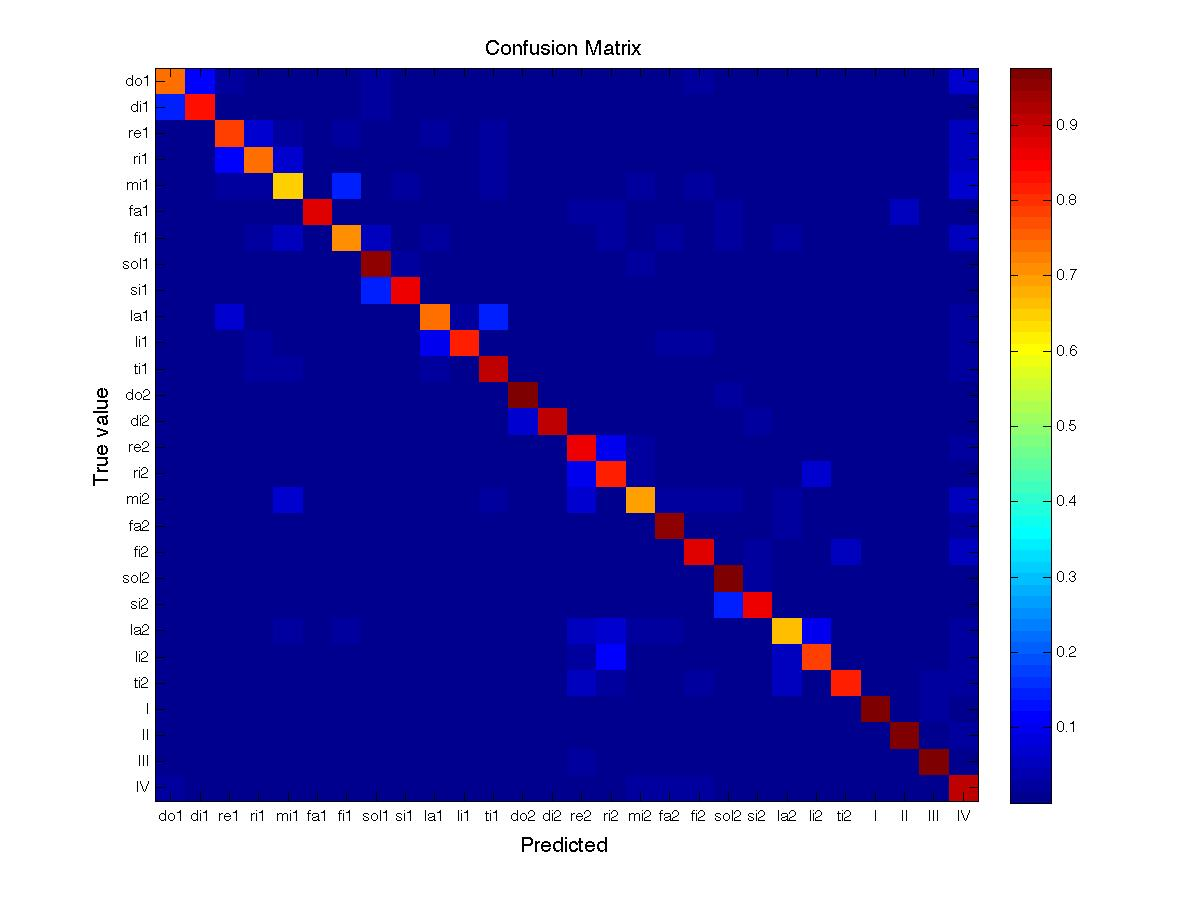
\includegraphics[width=\linewidth]{confmat/confusion.jpg}
	\caption{Confusion matrix using HOG, SVM $\chi^2$, n-fold, per film simple set}
	\label{fig:confusion}
\end{figure}




\subsection{Part II - evaluating Sonic Gesture}

\subsubsection{Method}

\begin{figure}[htbp]
\center{}
\subfloat[Without stabilizer]{
	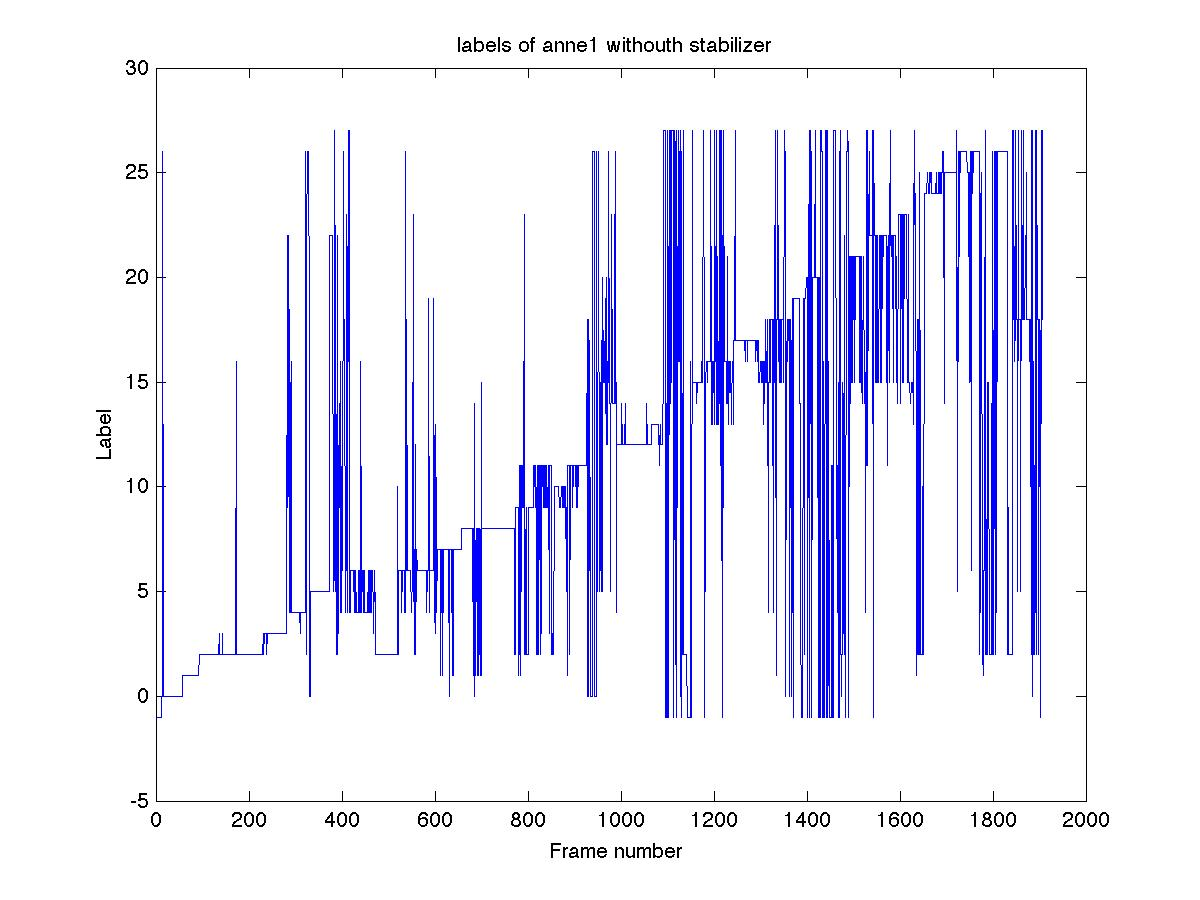
\includegraphics[width=0.3\linewidth]{figures/performance/anne1_unstable.jpg}}
\hspace{0.02\linewidth}
\subfloat[With stabilizer]{
	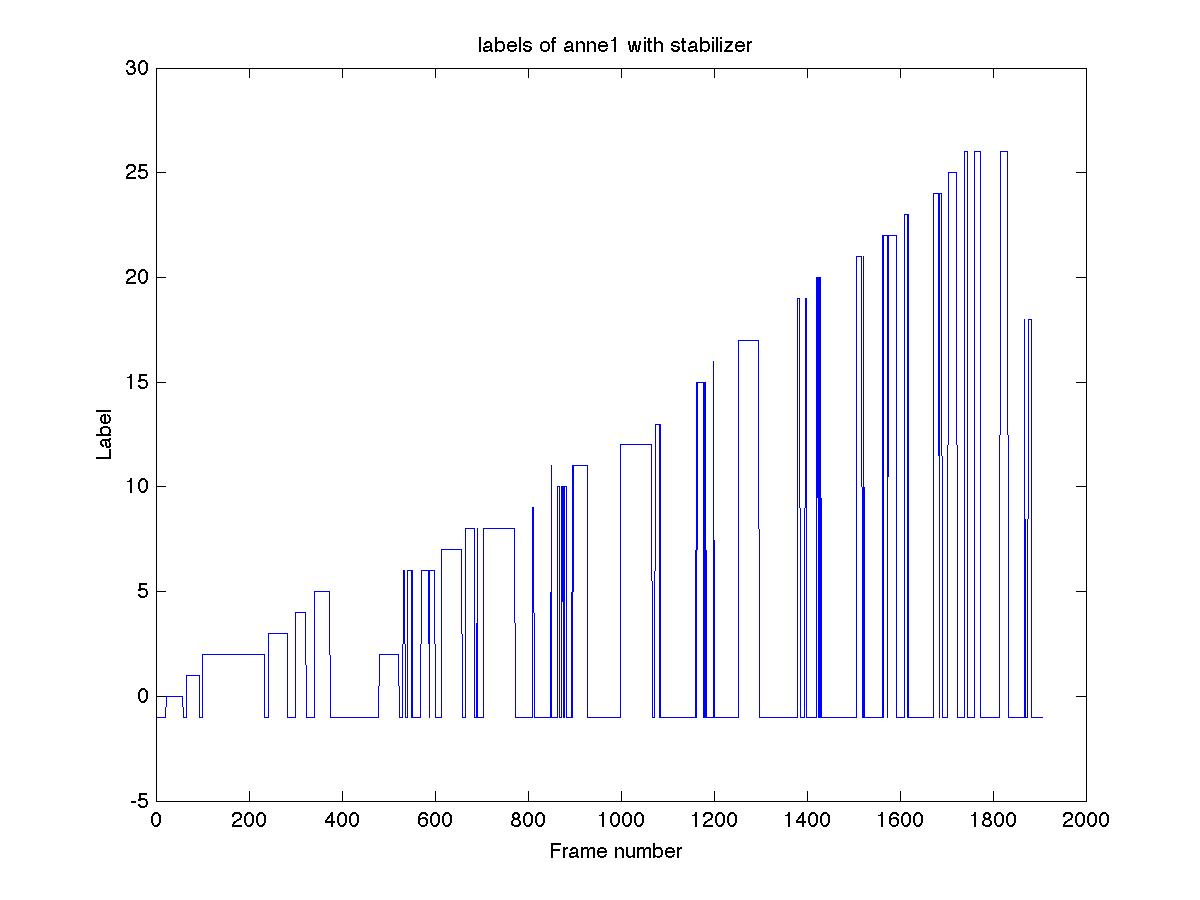
\includegraphics[width=0.3\linewidth]{figures/performance/anne1_stable.jpg}}
\hspace{0.02\linewidth}
\subfloat[Arbitrary movie with stabilizer]{
	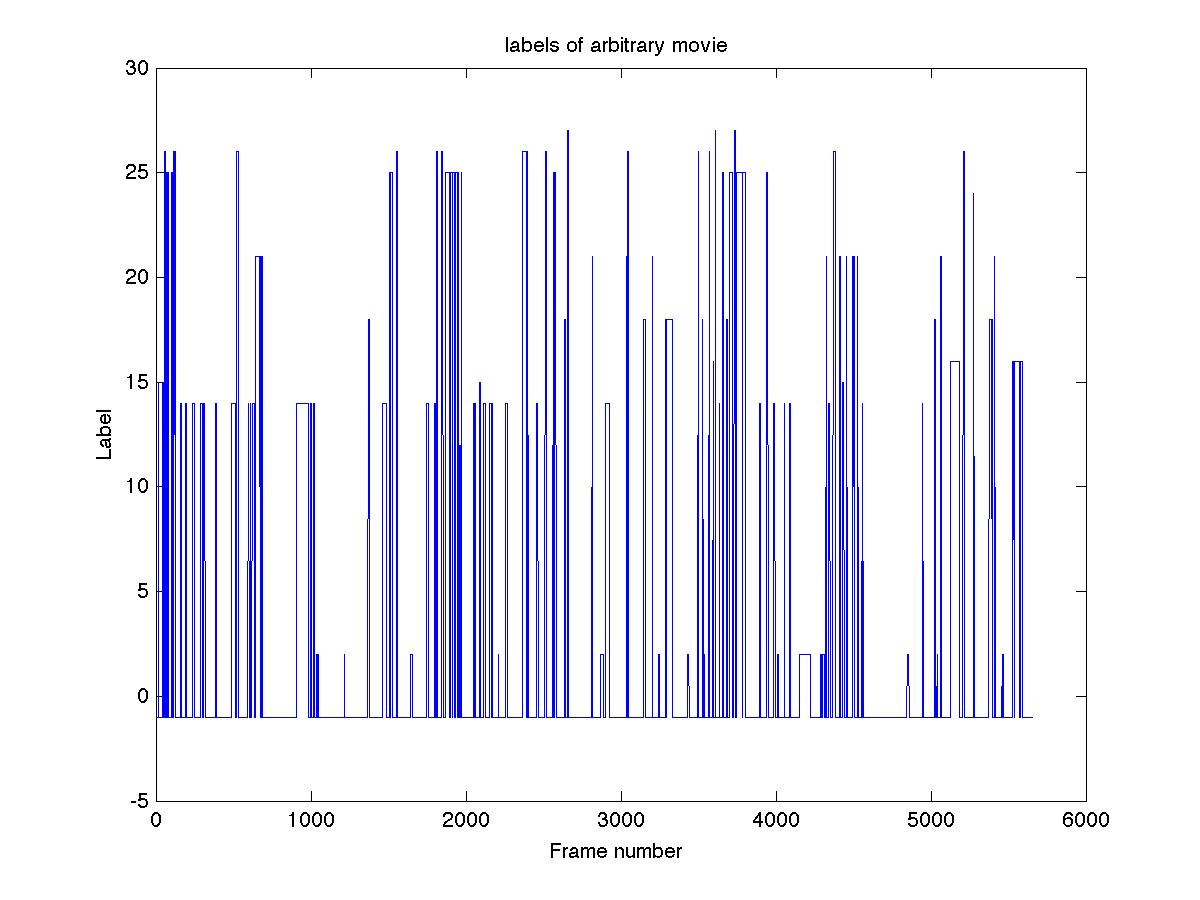
\includegraphics[width=0.3\linewidth]{figures/performance/heilige.jpg}}
\caption{Plots of labels per frame}
\label{fig:performances}
\end{figure}

To evaluate Sonic Gesture in the time domain, the sequential output must be evaluated. Sonic gesture outputs for every frame the estimated label for each hand. Constructing a ground truth for each frame is a difficult, time consuming and subjective process. The material is also 'polluted' with wrong hand poses caused by misunderstanding or misinterpretation. In some cases there are also more people in the image than only the test subject. To evade these problems a different evaluation method is used, where the consecutive changes in labels is evaluated. Since the goal for each recorded movie in the dataset was to record a person performing the 28 hand poses sequentially, the ground truth is a ordered list of all labels.

\autoref{fig:performances} visualized the sequence of labels in three cases, (a) when no stabilizer is used, a erratic pattern is the result. When the stabilizer is used (b) a more smooth incremental label pattern is visible. (c) shows the label sequence of an arbitrary movie. Scoring these patterns would be useful for comparison an tweaking. This can be done by calculating the Damerau-Levenshtein distance to the ground truth.

the output of Sonic Gesture for all movies is stored. This results in a long list of labels - one label for each frame - for each move. In each list all repeating labels are replaced with one instance of that label. This reduces the length of each list significantly. Now this list can be used to compute the Damerau-Levenshtein Distance.

The Damerau-Levenshtein Distance algorithm is shown in Algorithm~\autoref{alg:dameraulevenshtein}. The algorithm calculated to number of deletions, insertions, substitutions and transpositions required to transform one string into an other. The maximum number of operations is equal to the length of shortest string. Because of the ground truth's length of 28 the minimum will always be 28 or less. This way the distance can be safely normalized and divided by 28, so all distances can be easily compared.

\begin{algorithm}
\caption{DamerauLevenshteinDistance(str1, str2)}
\label{alg:dameraulevenshtein}
\begin{algorithmic}
   \REQUIRE a string str1
   \REQUIRE a string str2
   \ENSURE The distance between str1 and str2

   \medskip

   \FOR{$i = 1$ to lenStr1}
       \STATE $\mathbf{D}[i, 0] \Leftarrow i$
   \ENDFOR
   \FOR{$j = 1$ to lenStr2}
       \STATE $\mathbf{D}[0, j] \Leftarrow j$
   \ENDFOR
   \FOR{$i = 1$ to lenStr1}
       \FOR{$j = 1$ to lenStr2}
       		\IF{str1$_{i} =$ str2$_{j}$}
				\STATE cost $\Leftarrow 0$
            \ELSE
				\STATE cost $\Leftarrow 1$
			\ENDIF
			\STATE $x \leftarrow \mathbf{D}_{i-1, j  } + 1$ % deletion
			\STATE $y \leftarrow \mathbf{D}_{i  , j-1} + 1$ % insertion
            \STATE $z \leftarrow \mathbf{D}_{i-1, j-1} + $ cost % substitution
            \STATE $\mathbf{D}_{i, j} \Leftarrow \min(x, y, z)$
            \IF {(str1$_{i} =$ str2$_{j-1}$) $\wedge$ (str1$_{i-1} =$ str2$_{j}$)}
				\STATE $\mathbf{D}_{i, j} \Leftarrow \min(
                	\mathbf{D}_{i, j},
                    \mathbf{D}_{i-2, j-2} + $ cost  % transposition
                )
			\ENDIF
		\ENDFOR
	\ENDFOR
   \RETURN $\mathbf{D}_{lenStr1, lenStr2}$

\end{algorithmic}
\end{algorithm}
	
\subsubsection{Results}
\autoref{tab:distance} contains all distances, grouped per dataset. The numbers in table heading are the movie number of that column. The average column is the \textit{average} of all movies per person. The average per person column lists the same distances, but without using the stabilizer discussed in \autoref{subsec:stabilizer}. As you see this has a dramatic impact on the performance. The average distance for the simple set is 0.27, for the complex set 0.35. 



\begin{table}
\centering
\begin{tabular}{p{0.4in}rrrrrrrp{0.55in}}
\hline
Dataset & Name	& 1 & 2 & 3 & 4 & 5 & Average & Average without stabilizer\\
\hline
Simple & Anne	&	0.43	&	0.32	&	0.25	&	0.29	&	0.14	&	0.28	&	0.88 \\
 & Arjan	&	0.46	&	0.25	&	0.25	&	0.07	&	0.29	&	0.26	&	0.83 \\
 & Gijs	&	0.14	&	0.18	&	0.21	&	0.21	&	0.14	&	0.18	&	0.87 \\
 & Ivo	&	0.07	&	0.11	&	0.07	&	0.11	&	0.04	&	0.08	&	0.86 \\
 & Jasper 1	&	0.68	&	0.46	&	0.21	&	0.21	&	0.43	&	0.40	&	0.85 \\
 & Peter	&	0.25	&	0.29	&	0.25	&	0.32	&	0.18	&	0.26	&	0.86 \\
 & Hanne	&	0.32	&	0.00	&	0.04	&	0.25	&	0.07	&	0.14	&	0.91 \\
 & Jasper 2	&	0.32	&	0.18	&	0.18	&	 	&	 	&	0.23	&	0.90 \\
 & Ork	&	0.21	&	0.18	&	0.14	&	 	&	 	&	0.18	&	0.86 \\
 & Roberto	&	0.68	&	0.29	&	0.46	&	 	&	 	&	0.47	&	0.83 \\
 & Xirong	&	0.61	&	0.50	&	0.36	&	 	&	 	&	0.49	&	0.88 \\
\hline
Complex & Gosia	&	0.57	&	0.32	&	0.21	&	 	&	 	&	0.37	&	0.88 \\
 & Hamdi	&	0.50	&	0.43	&	0.54	&	 	&	 	&	0.49	&	0.87 \\
 & Michael	&	0.21	&	0.29	&	0.46	&	 	&	 	&	0.32	&	0.90 \\
 & Sil	&	0.50	&	0.61	&	0.46	&	 	&	 	&	0.52	&	0.83 \\
 & Victoria	&	0.32	&	0.21	&	0.18	&	 	&	 	&	0.24	&	0.88 \\
 & Chu	&	0.29	&	0.21	&	0.07	&	 	&	 	&	0.19	&	0.89 \\
\hline
Complex & Koen	&	0.39	&	0.32	&	0.39	&	 	&	 	&	0.38	&	0.88\\
with & Bas	&	0.54	&	0.43	&	0.32	&	 	&	 	&	0.44	&	0.90 \\
poster & Stratis	&	0.43	&	0.11	&	0.18	&	 	&	 	&	0.24	&	0.86 \\


\hline
\end{tabular}
\caption{Damerau-Levenshtein distance of all movies}
\label{tab:distance}
\end{table}



\subsection{Part III - The Search for Spock}

\subsubsection{Method}
To show that Sonic Gesture can also work with non artificial video material a third experiment was constructed. For this experiment a collection of real fragments of movies and pictures of people performing the 'Vulcan Salute' was gathered. The Vulcan Salute is greeting hand gesture and was popularised by the half-Vulcan character Mr. Spock on the Star Trek television series in end of the 1960s. \autoref{fig:spock} is a movie fragment of Mr. Spock giving the hand salute. The original dataset used for the previous experiments was extended with a 29th hand pose, the vulcan salute. 

\begin{figure}[htbp]
\centering{}
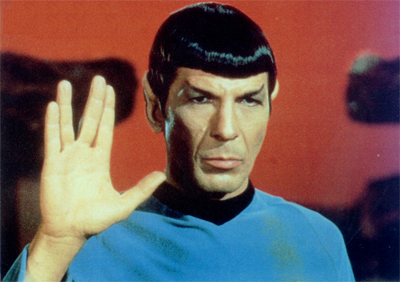
\includegraphics[width=0.6\linewidth]{figures/spock/salute.png}
\caption{Mr. Spock giving the Vulcan Salute}
\label{fig:spock}
\end{figure}


\subsubsection{Results}
\autoref{fig:vulcangood} shows eight examples of successful classification of the vulcan salute. The images are cutout screenshots of the implementation of Sonic Gesture. The upper left window is the input, the upper right window is the segmented and labeled visualisation. A green square indicates a right hand and yellow left. The bottom squares show the estimated hand poses, the left square for the left hand and the right square for the right hand. For the visualisation of the detected Vulcan Salute the picture of Mr. Spock is used.

\autoref{fig:vulcanfail} shows two screenshots of failed segmentation. Sonic Gesture fails on the first salute - performed by Condolisa Rise - because the skin segmentation fails. The skin colour of her face has more in common with the wall than with her hand. The second failure case is performed by Simon Pegg, here the segmentation is correct, but classification is just wrong. More training data could fix this problem.

\begin{figure}[htbp]
\centering
\subfloat{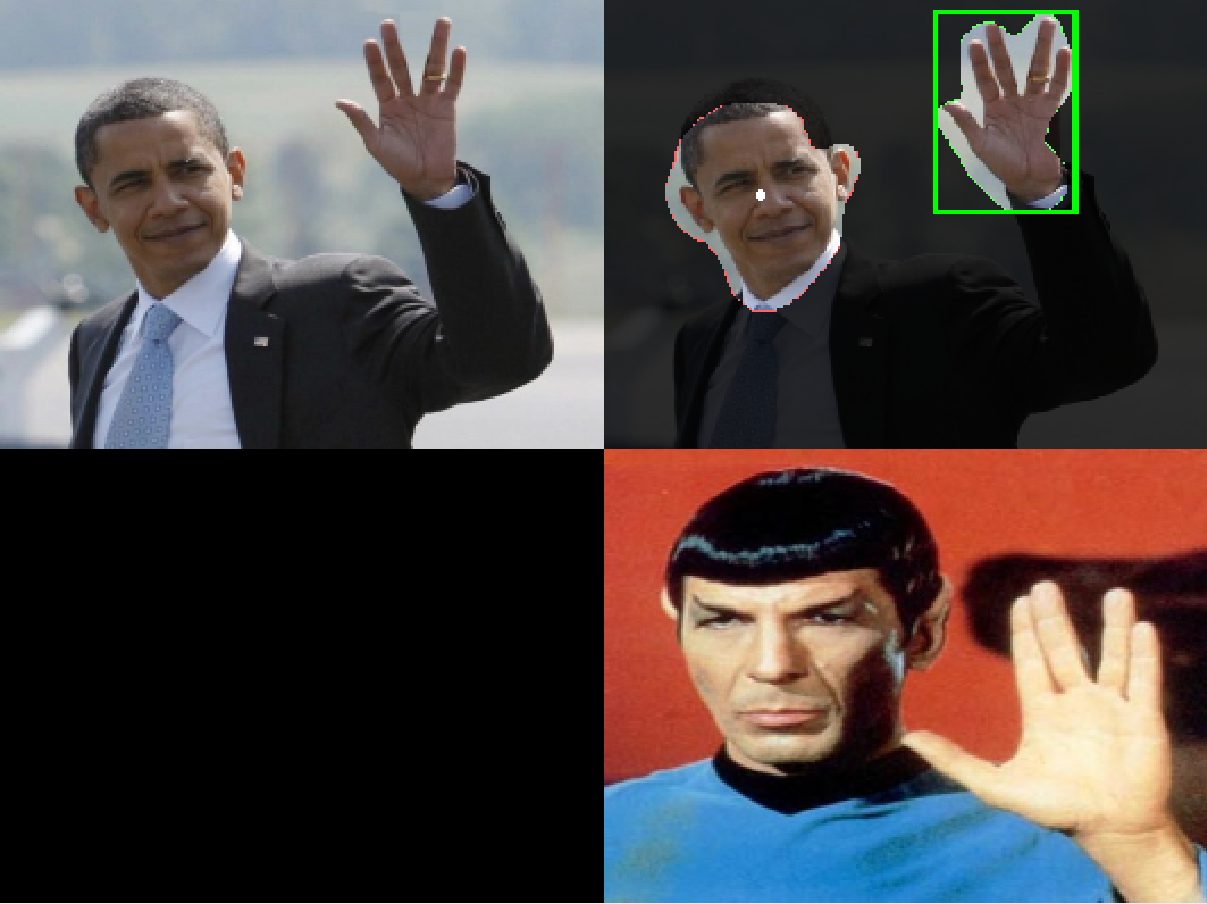
\includegraphics[width=0.45\linewidth,height=0.35\linewidth]{figures/spock/good1.png}}
\hspace{0.09\linewidth}
\subfloat{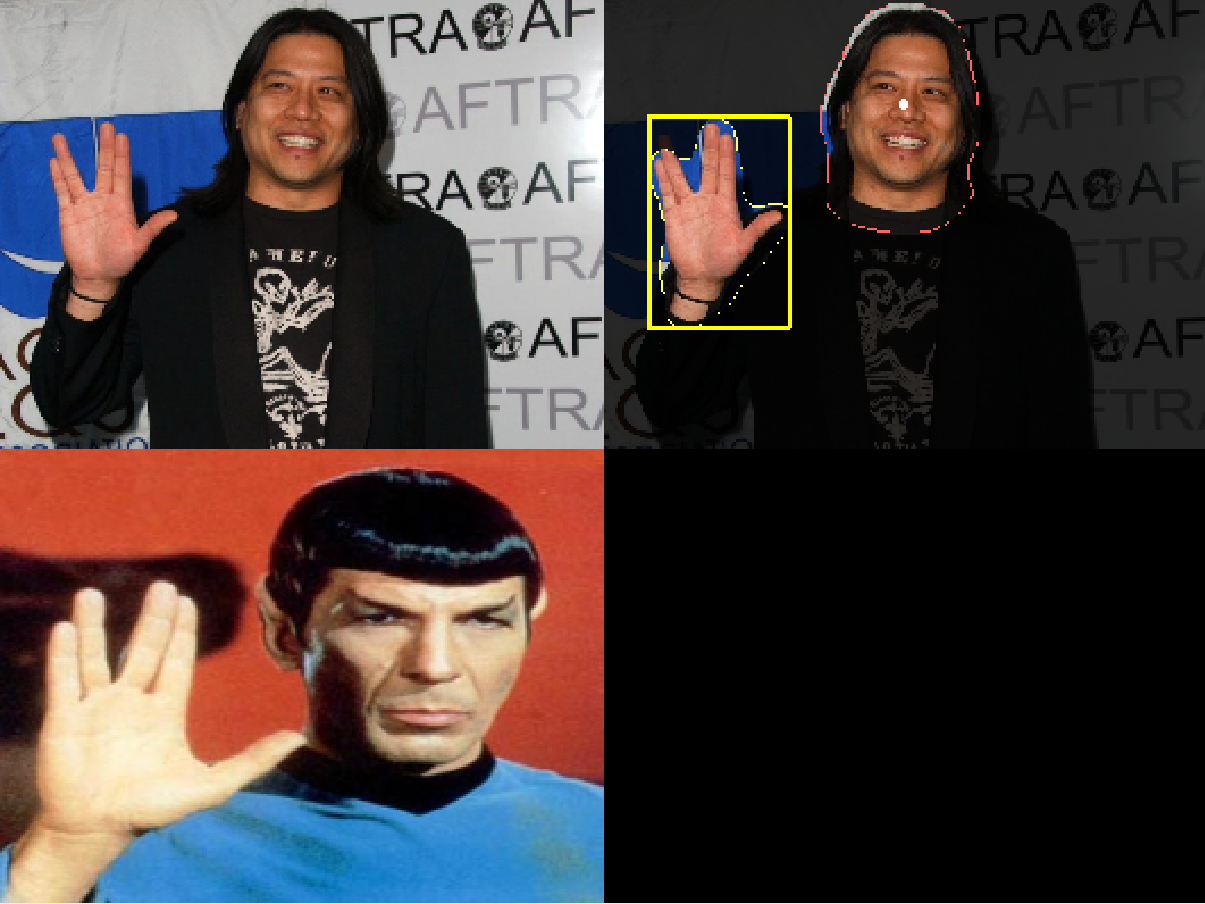
\includegraphics[width=0.45\linewidth,height=0.35\linewidth]{figures/spock/good2.png}}
\hspace{0.09\linewidth}
\subfloat{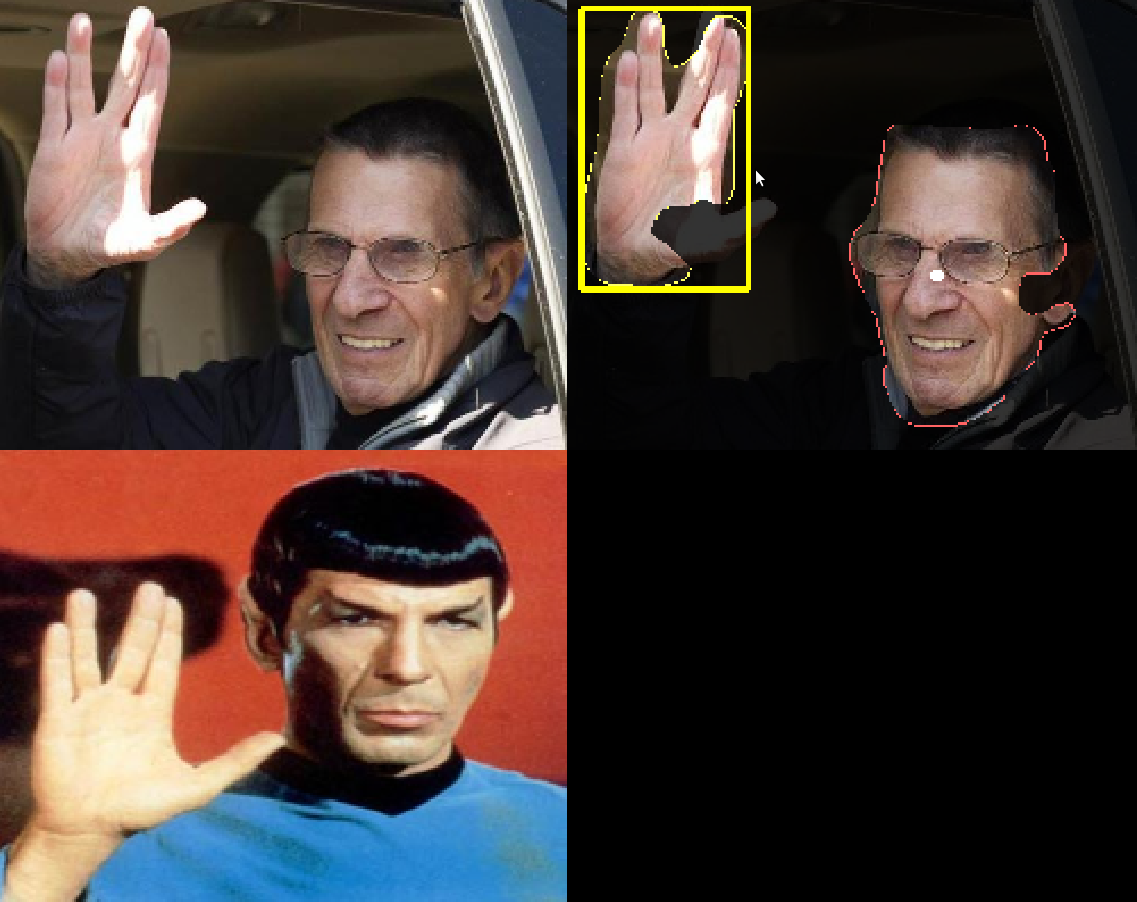
\includegraphics[width=0.45\linewidth,height=0.35\linewidth]{figures/spock/good3.png}}
\hspace{0.09\linewidth}
\subfloat{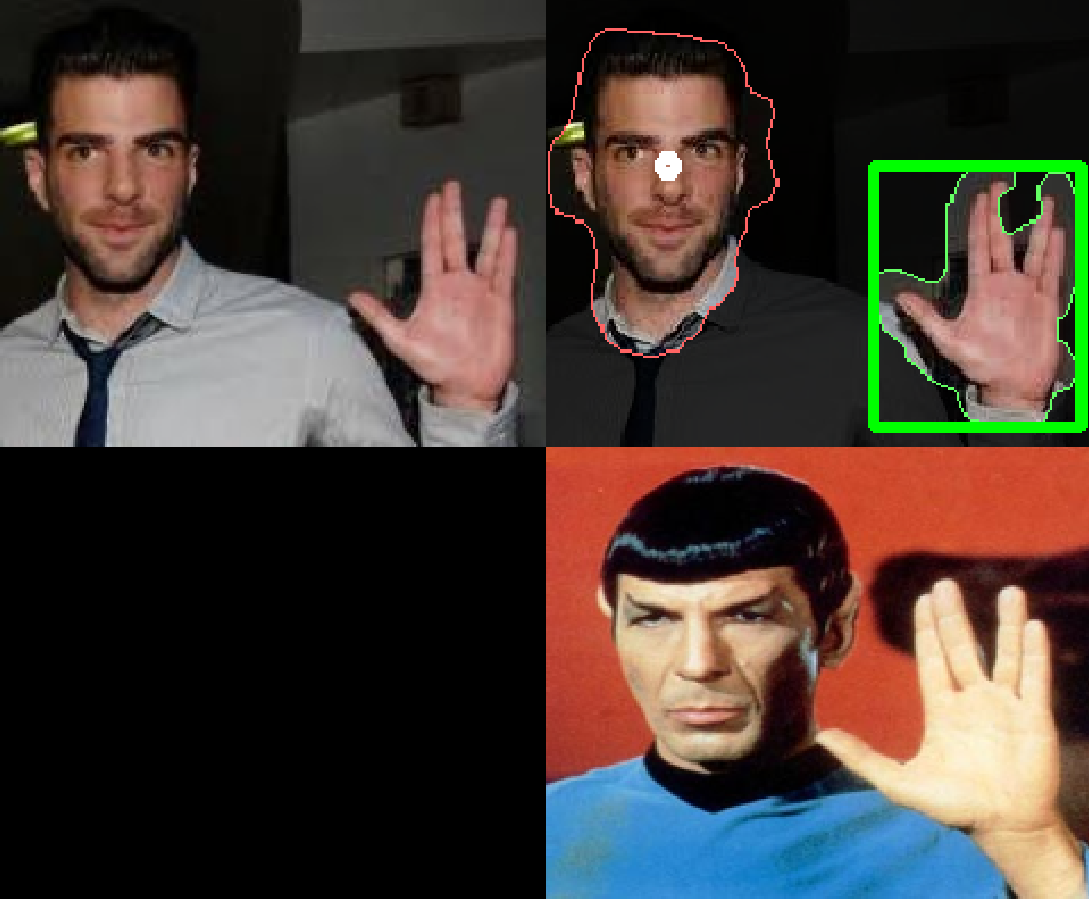
\includegraphics[width=0.45\linewidth,height=0.35\linewidth]{figures/spock/good4.png}}
\hspace{0.09\linewidth}
\subfloat{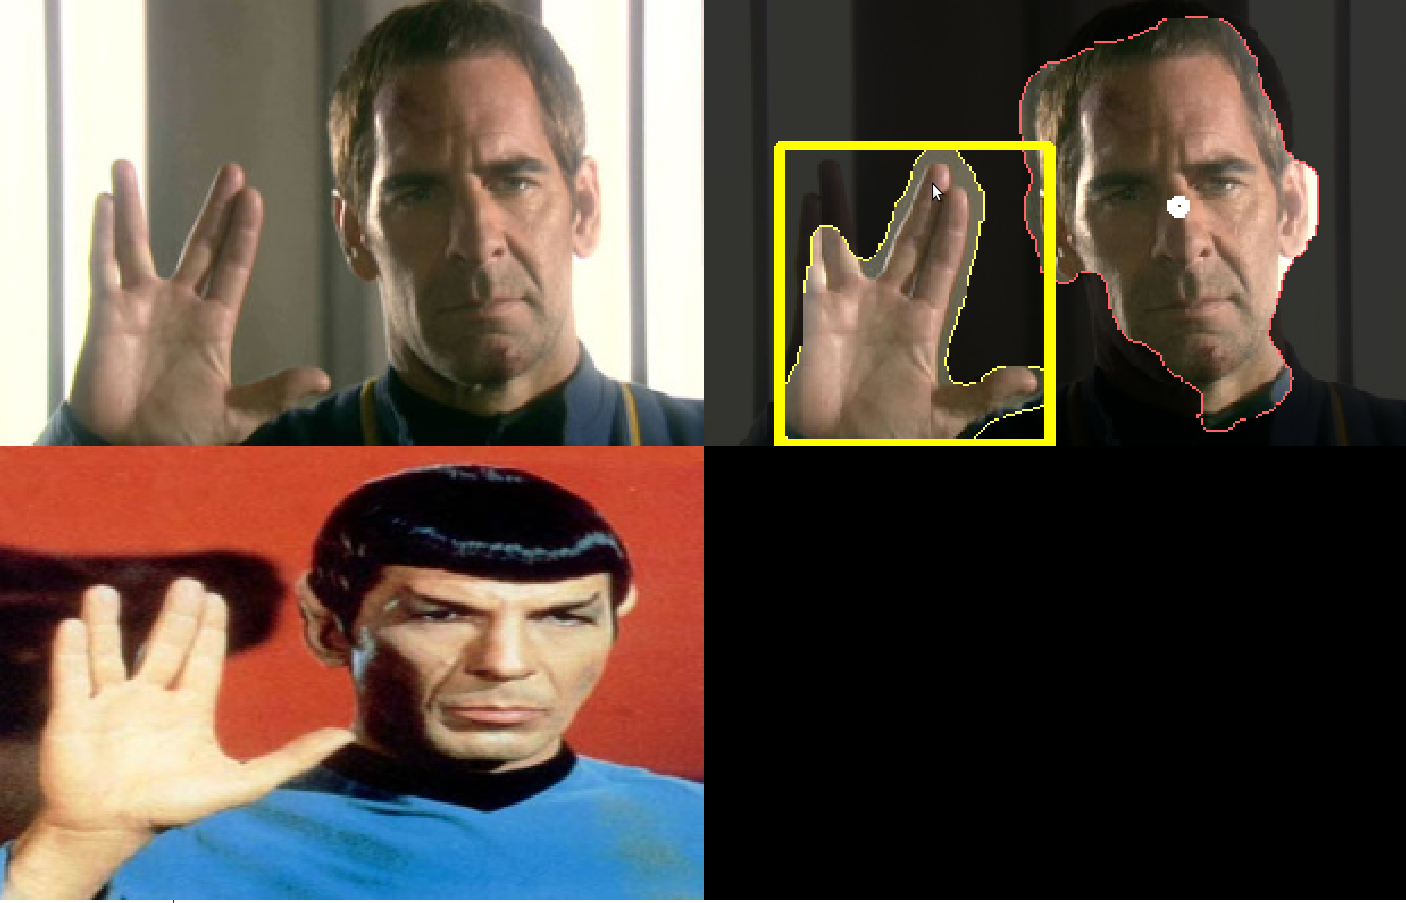
\includegraphics[width=0.45\linewidth,height=0.35\linewidth]{figures/spock/good5.png}}
\hspace{0.09\linewidth}
\subfloat{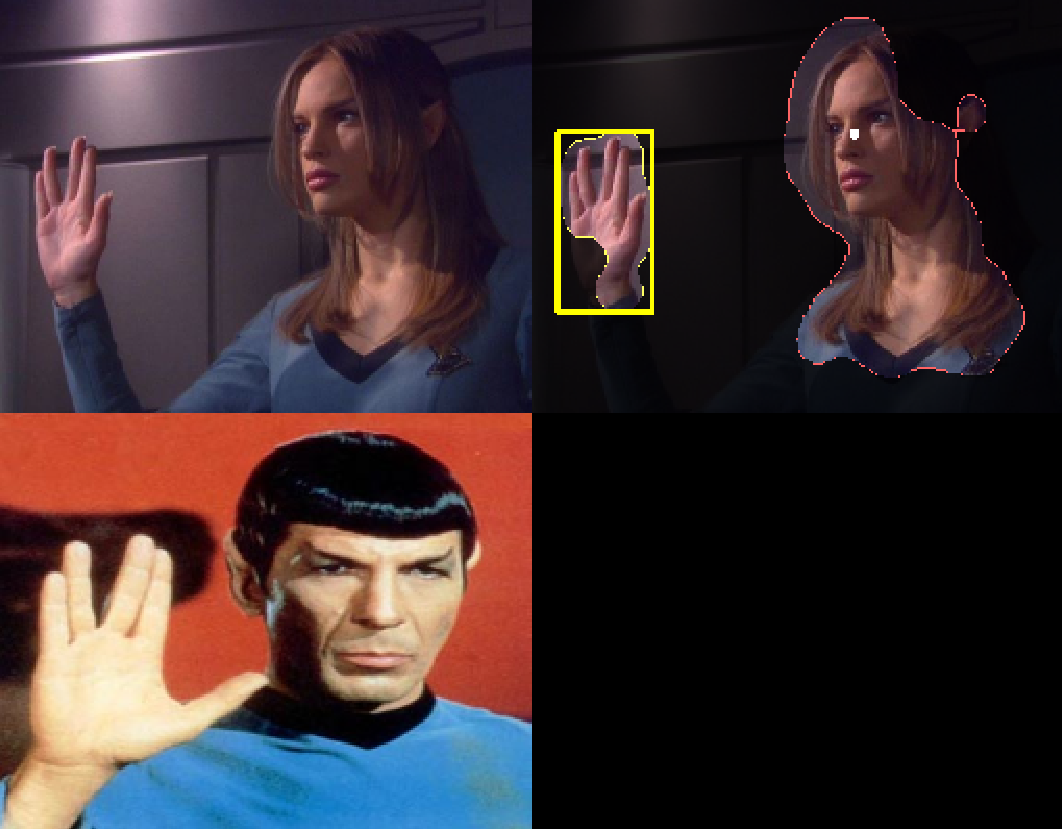
\includegraphics[width=0.45\linewidth,height=0.35\linewidth]{figures/spock/good6.png}}
\hspace{0.09\linewidth}
\subfloat{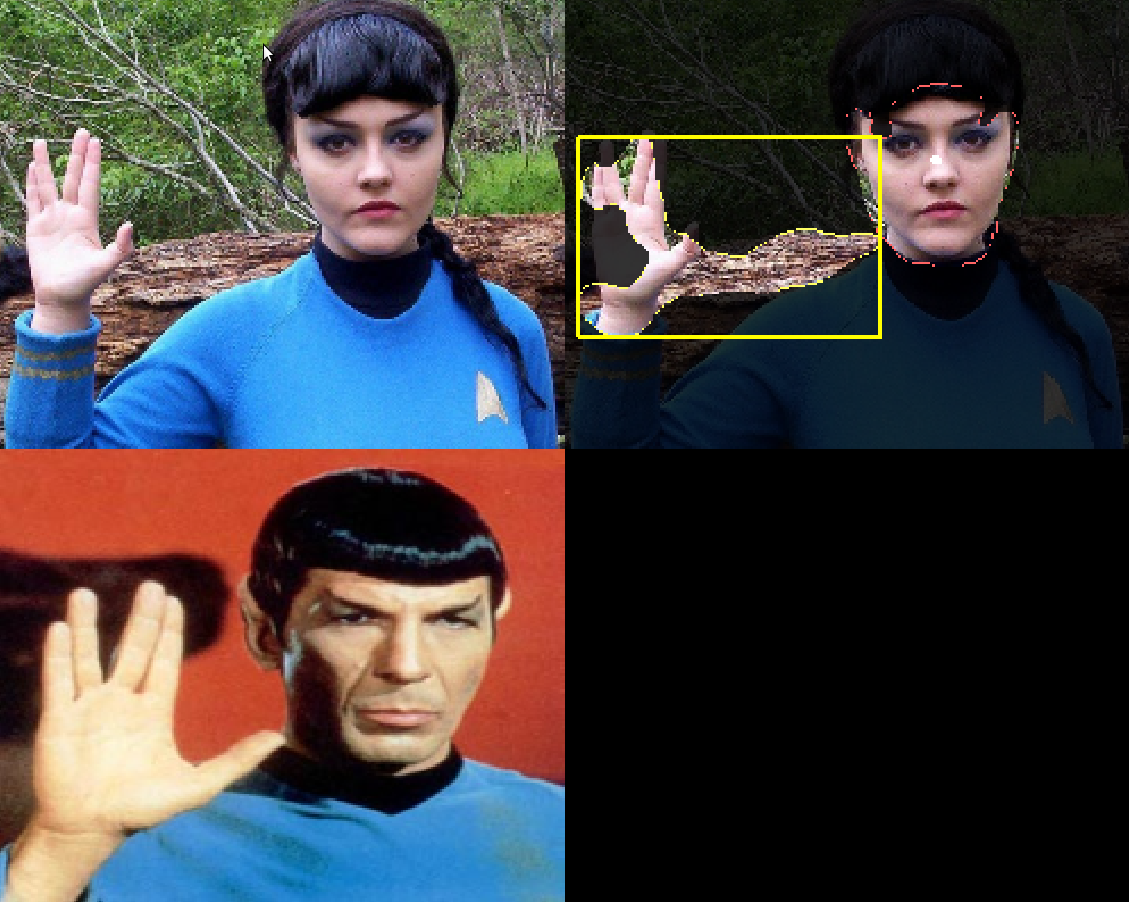
\includegraphics[width=0.45\linewidth,height=0.35\linewidth]{figures/spock/good7.png}}
\hspace{0.09\linewidth}
\subfloat{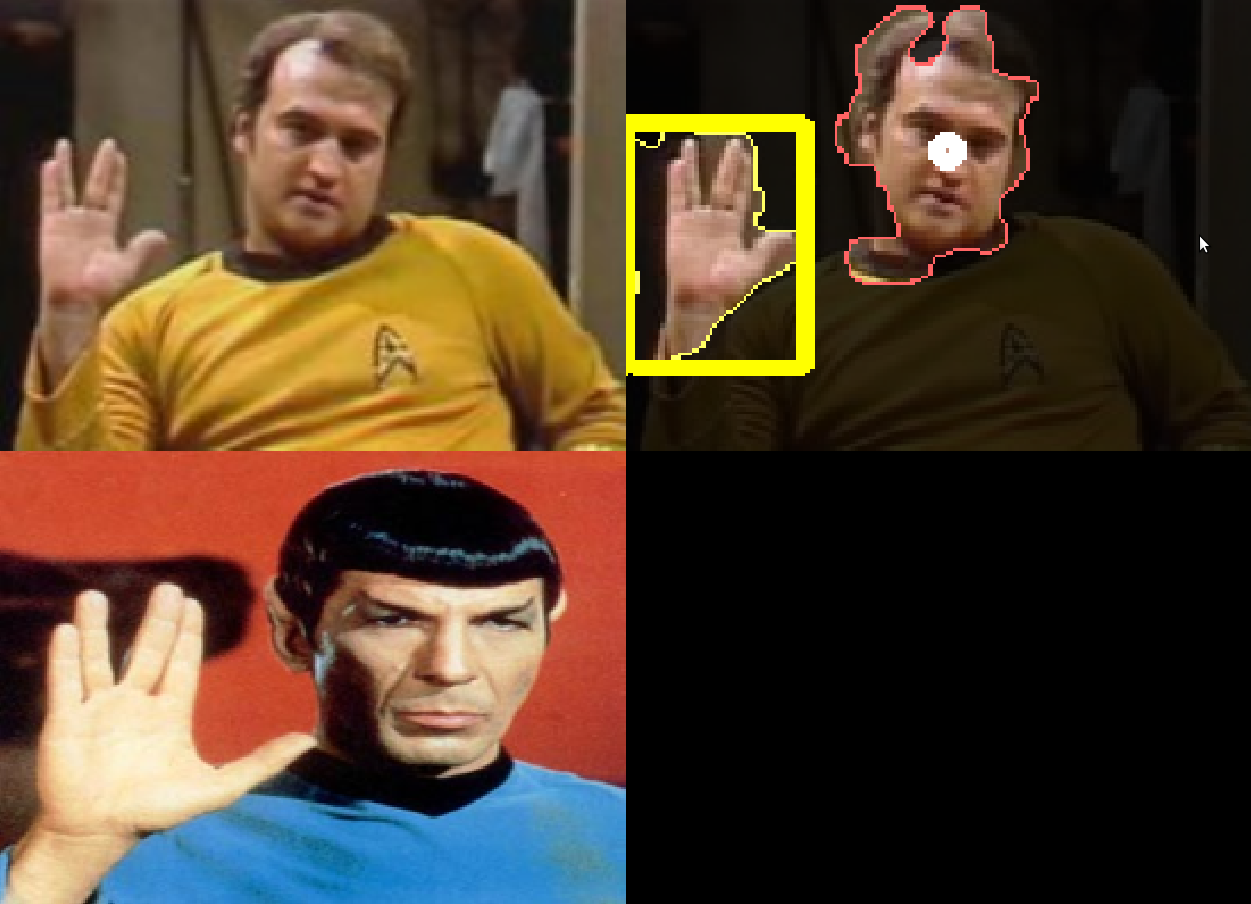
\includegraphics[width=0.45\linewidth,height=0.35\linewidth]{figures/spock/good8.png}}
\hspace{0.09\linewidth}
\caption{Successful detection of Vulcan salute}
\label{fig:vulcangood}
\end{figure}


\begin{figure}[htbp]
\centering
\subfloat{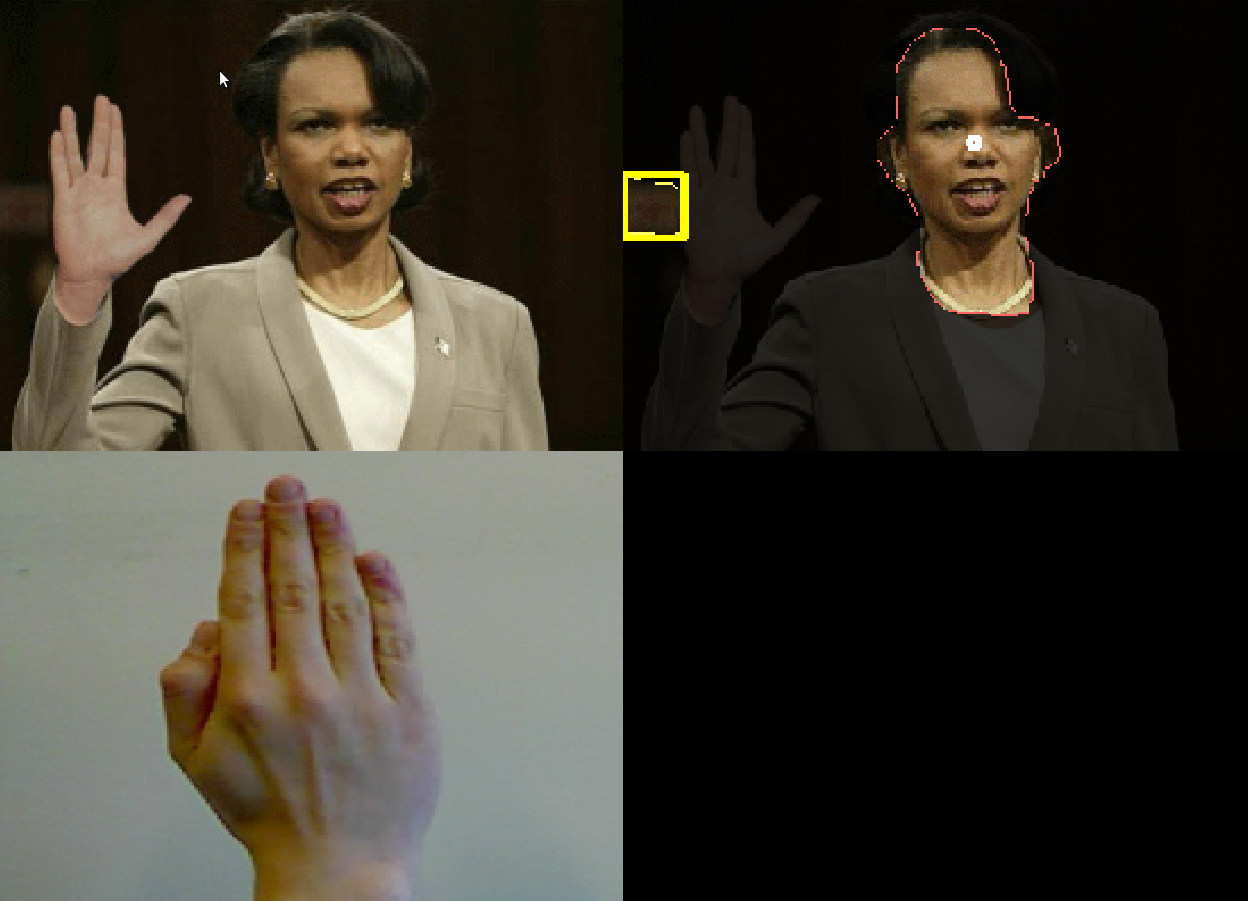
\includegraphics[width=0.45\linewidth,height=0.35\linewidth]{figures/spock/fail1.png}}
\hspace{0.09\linewidth}
\subfloat{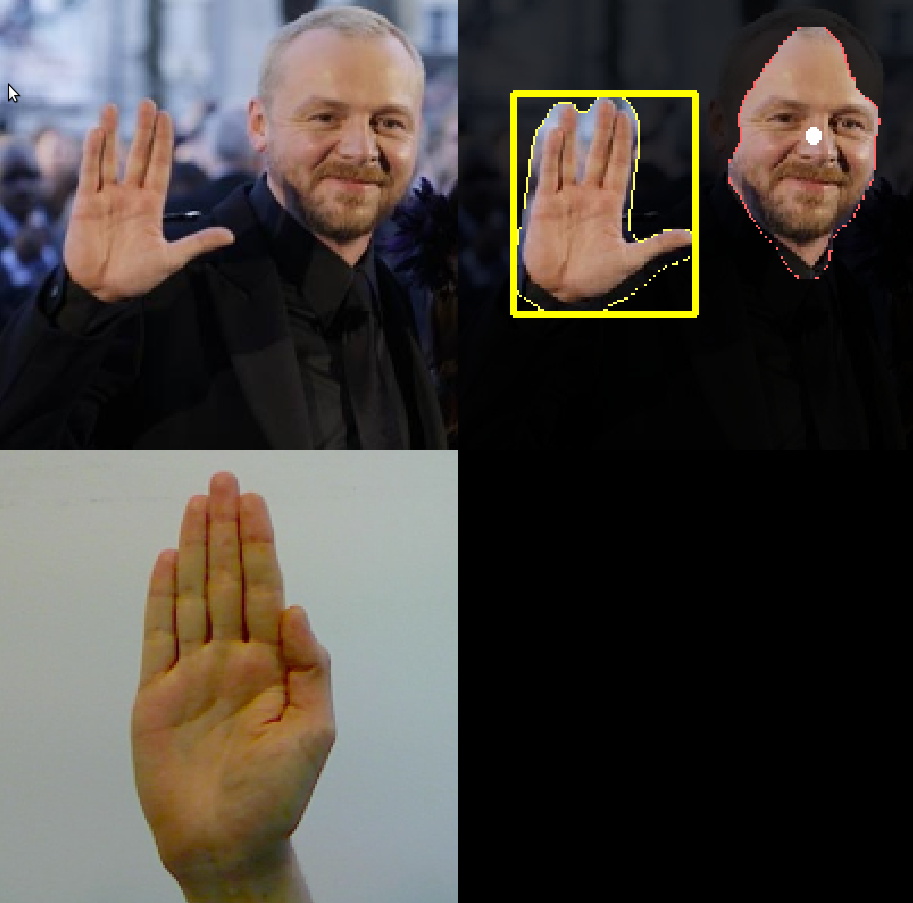
\includegraphics[width=0.45\linewidth,height=0.35\linewidth]{figures/spock/fail2.png}}
\caption{Failed detection of Vulcan salute}
\label{fig:vulcanfail}
\end{figure}




%!TEX root = thesis.tex

\chapter{Sonic Gesture}
\label{ch:sonicgesture}

\section{Implementation}
\label{sec:implementation}

\begin{figure}[ht]
\centering{}
\includegraphics[width=0.6\linewidth]{figures/sonicgesture.jpg}
\caption{Screenshot of Sonic Gesture}
\label{fig:sonicgesture}
\end{figure}

Sonic Gesture has been implemented in C++. Almost all computer vision algorithms used are part of OpenCV, an open source library made for this kind of software. For the graphical interface QT is used. Sonic Gesture has been release as Open Source software and is released under the Apache license. The software can be downloaded, modified and distributed freely from the website\footnote{http://code.google.com/p/sonic-gesture}.

\autoref{fig:sonicgesture} is a screenshot of the main screen of sonic gesture. The program can capture directly from a webcam or it can read movies with recorded material. It has 2 modes, the first is the `finder' mode where hand poses in the video stream are detected and classified. The second mode is the `capture' mode, which is used to label movies. When labeling a movie in this mode a text file is created with frame positions of the labels. This can later be used to extract the correct frame and extract training data for the classifier. This mode has been used a lot during the gathering of the dataset.

When the finder mode is active, Sonic Gesture will translate the labeled hand poses, the hand positions and the size of the hand into Open Sound Control (OSC). OSC is a protocol which is specifically designed for transferring audio information over a network. For those who are familiar with digital music, it is very similar to MIDI. A program that can interpreted OSC can then be configured to listen on a specific port and process these OSC command.

Sonic Gesture will submit
\begin{itemize}
	\item For each hand the beginning and the end of detected sequence of hand specific hand pose. This is an integer. This can be used to trigger a action, like playing a specific note.
	\item The position of each hand in $x$ and $y$ position. This is a float and can be used to manipulate a parameter.
	\item The size of the hand. This is also a float and can also be used to manipulate a parameter.
\end{itemize}

There is no strict defined relationship between a hand pose and a sound or parameter, the user of Sonic Gesture can define his own specific mapping with his or her preferred audio application. 

\begin{figure}[ht]
\centering{}
\includegraphics[width=0.9\linewidth]{figures/sonicableton.png}
\caption{Sonic Gesture linked to Ableton with OSCulator}
\label{fig:sonicableton}
\end{figure}

\section{Time Performance}
A lot of effort has been put into getting Sonic Gesture as fast as possible. Initially Sonic Gesture was written in Python and used the Python API of OpenCV. Soon it became clear that Python was to limited to do high performance graphic processing so a switch to C++ was made. 

The performance of Sonic Gesture depends on how fast the testing systems CPU power is, if the OpenCV IPP extensions is used, but also how fast the camera can capture frames. On a Macbook Pro, 2.4 GHz intel core 2 duo with 4 GB of memory using the build-in iSight as camera, processing one frame takes 65 ms on average. This is with the full dataset of 2072 datapoints with 3780 dimensions using the KNN classifier. KNN works fine with low numbers of datapoint, but with high numbers it starts to slow down. Still it is quite fast; around 25 ms on average. SVM will probably perform much faster with a high number of datapoints but we couldn't get the SVM implementation of OpenCV to work. An other expensive operation is the face detection algorithm, when tweaked it takes around 13 ms to locale a face in a image. Since a face position is not required constantly this is done only every 10th frame, so valuable computation time is saved. An other surprisingly expensive operation is the resizing of a image. Resizing an image to a small size is a crucial part of the pipe line, because some operations on a big image will take too much time. But resizing a image using interpolation is a expensive operation. Where interpolation is not required, for example for rendering on the screen, it is disabled saving more computing time. 



\begin{table}
\centering
\begin{tabular}{ccc}
What & relative time & comment \\
\hline
kNN & 47\% & 3780 features, 2016 samples \\
Color space convertion & 8.4\% & \\
Image resizing & 7.6\% & \\
Face detection & 3.7\% &  19\% if every frame \\
HOG features & 2.6\% \\
\end{tabular}
\caption{Performance timing of Sonic Gesture}
\end{table}

calculating SURF features of a hand train image takes 4ms and results in 11 features on average.

%!TEX root = thesis.tex

\chapter{Conclusions}
\label{ch:conc}
A method is proposed, implemented and evaluated for performing real-time computer vision based hand pose extraction with a single RGB camera and could run on current consumer level computing power. The implementation shows that the system is usable in a real-time human computer interaction setting, e.g. used for creating and manipulating sound. It is assumed that in the input video stream only one person is visible, this person is wearing clothing with long sleeves, and no skin-like colors are in the image.

The implementation uses a histogram based probabilistic skin color model which is based upon the users face which is found by a haar classifier. This is a robust way for face detection and the detection speed is reasonable if performed every 10th frame. The face detection will give unpredictable results when multiple faces are visible in the input image.

The skin color model is an effective and fast way to localize body parts in the image, but it is required that no skin-like colors are in the input image. Going from the probabilistic domain to the labeled binary domain can be controlled with a threshold parameter.  This parameter can be automatically adjusted, but a carefully chosen fixed value is enough for most cases. 

Using heuristics for blob labeling is a robust method, but fails when the hands cross their position in the $x$ direction. Keeping the labels of a blob fixed after the first detection could solve this problem, but introduce many new problems like what to do when the blobs are gone for sequence of frames and decide at what moment a blob should get which label.

Using HOG features for image representation gave very good results, much better than SURF features. This is probably caused by the improper use of SURF, where the use of the keypoint detection phase seems essential. In the experiments HOG and SURF where both used with a dense grid of keypoints.

$k$-NN can be used as a classifier, but becomes slow when a lot of training samples (+2000) are used. SVM is a better alternative, which yields better performance in classification time an accuracy. As a kernel for SVM the $\chi^2$ and RBF kernel accomplish similar results, but the RBF kernel requires the optimization of one extra parameter $\gamma$. This extra parameter requires more work during the training phase, so the $\chi^2$ kernel is preferred.

Even though the accuracy of the classification system was high in some benchmarks, the choice of the Curwen hand poses as `language' wasn't a good one. A smaller set with hand poses that are less similar and have a large visible surface would perform better.

The experiment results show that the system is not person independent. Incorporating training data gathered from the eventual user will improve the classification performance. It is not yet known if the performance will increase with more training data. Also the best results are yielded when a simple background is used.

\section{Future Work}
The performance of the system could be evaluated when configured with less hand poses that are less similar. Also the current dataset is to small to analyze the impact of more or less train data. A bigger dataset could be constructed and the impact on person independence could be studied.

Less scientific but also interesting is the things that could be done with the implementation of Sonic Gesture. It currently uses the $k$-NN classifier, but the experiments show that a SVM classifier with the $x^2$ kernel perform much better. Currently it doesn't use automatic threshold adjusting, something that can be implemented also. The capture mode is currently not very user friendly, something that would help gathering train data when improved. 


\cleardoublepage
\phantomsection
\addcontentsline{toc}{chapter}{Bibliography}
\bibliography{thesis}
\bibliographystyle{plainnat}


%!TEX root = thesis.tex

\appendix

\chapter{Images}

\begin{figure}[tb]
\begin{center}
\subfloat[input frame]{\label{fig:pipe_input}\includegraphics[width=0.3\linewidth]{figures/pipeline/input.jpg}}
\hspace{0.03\linewidth}
\subfloat[hue channel]{\label{fig:hue2}\includegraphics[width=0.3\linewidth]{figures/pipeline/hue.jpg}}
\hspace{0.03\linewidth}
\subfloat[saturation channel]{\label{fig:saturation2}\includegraphics[width=0.3\linewidth]{figures/pipeline/saturation.jpg}}
\hspace{0.03\linewidth}
\subfloat[value channel]{\label{fig:value2}\includegraphics[width=0.3\linewidth]{figures/pipeline/value.jpg}}
\hspace{0.03\linewidth}
\subfloat[face detection]{\includegraphics[width=0.3\linewidth]{figures/pipeline/detected.jpg}}
\hspace{0.03\linewidth}
\subfloat[Face color histogram]{\label{fig:pipe_hist}\includegraphics[width=0.3\linewidth]{figures/pipeline/histogram.png}}
\hspace{0.03\linewidth}
\subfloat[Backprojection]{\label{fig:pipe_bp}\includegraphics[width=0.3\linewidth]{figures/pipeline/backproject.jpg}}
\hspace{0.03\linewidth}
\subfloat[Gaussian smooth]{\label{fig:pipe_blur}\includegraphics[width=0.3\linewidth]{figures/pipeline/blurred.jpg}}
\hspace{0.03\linewidth}
\subfloat[Thresholded binary image]{\label{fig:pipe_th}\includegraphics[width=0.3\linewidth]{figures/pipeline/thresholded.jpg}}
\hspace{0.03\linewidth}
\subfloat[Morpholoical close]{\label{fig:pipe_close}\includegraphics[width=0.3\linewidth]{figures/pipeline/closed.jpg}}
\hspace{0.03\linewidth}
\subfloat[Blob labeling]{\label{fig:pipe_cont}\includegraphics[width=0.3\linewidth]{figures/pipeline/contours.jpg}}
\end{center}
\caption{The complete hand pose detection pipeline}
\label{fig:pipeline}
\end{figure}


\renewcommand{\thesubfigure}{\thefigure.\roman{subfigure}}
\begin{figure}[tb]
\begin{center}
\subfloat[Do]{\label{fig:hand_0}\includegraphics[width=0.2\linewidth,height=0.15\linewidth]{figures/examples/0.jpg}}
\hspace{0.03\linewidth}
\subfloat[Di]{\label{fig:hand_1}\includegraphics[width=0.2\linewidth,height=0.15\linewidth]{figures/examples/1.jpg}}
\hspace{0.03\linewidth}
\subfloat[Re]{\label{fig:hand_2}\includegraphics[width=0.2\linewidth,height=0.15\linewidth]{figures/examples/2.jpg}}
\hspace{0.03\linewidth}
\subfloat[Ri]{\label{fig:hand_3}\includegraphics[width=0.2\linewidth,height=0.15\linewidth]{figures/examples/3.jpg}}
\hspace{0.03\linewidth}
\subfloat[Mi]{\label{fig:hand_4}\includegraphics[width=0.2\linewidth,height=0.15\linewidth]{figures/examples/4.jpg}}
\hspace{0.03\linewidth}
\subfloat[Fa]{\label{fig:hand_5}\includegraphics[width=0.2\linewidth,height=0.15\linewidth]{figures/examples/5.jpg}}
\hspace{0.03\linewidth}
\subfloat[Fi]{\label{fig:hand_6}\includegraphics[width=0.2\linewidth,height=0.15\linewidth]{figures/examples/6.jpg}}
\hspace{0.03\linewidth}
\subfloat[Sol]{\label{fig:hand_7}\includegraphics[width=0.2\linewidth,height=0.15\linewidth]{figures/examples/7.jpg}}
\hspace{0.03\linewidth}
\subfloat[Si]{\label{fig:hand_8}\includegraphics[width=0.2\linewidth,height=0.15\linewidth]{figures/examples/8.jpg}}
\hspace{0.03\linewidth}
\subfloat[La]{\label{fig:hand_9}\includegraphics[width=0.2\linewidth,height=0.15\linewidth]{figures/examples/9.jpg}}
\hspace{0.03\linewidth}
\subfloat[Li]{\label{fig:hand_10}\includegraphics[width=0.2\linewidth,height=0.15\linewidth]{figures/examples/10.jpg}}
\hspace{0.03\linewidth}
\subfloat[Ti]{\label{fig:hand_11}\includegraphics[width=0.2\linewidth,height=0.15\linewidth]{figures/examples/11.jpg}}
\hspace{0.03\linewidth}
\subfloat[Do]{\label{fig:hand_12}\includegraphics[width=0.2\linewidth,height=0.15\linewidth]{figures/examples/12.jpg}}
\hspace{0.03\linewidth}
\subfloat[Di]{\label{fig:hand_13}\includegraphics[width=0.2\linewidth,height=0.15\linewidth]{figures/examples/13.jpg}}
\hspace{0.03\linewidth}
\subfloat[Re]{\label{fig:hand_14}\includegraphics[width=0.2\linewidth,height=0.15\linewidth]{figures/examples/14.jpg}}
\hspace{0.03\linewidth}
\subfloat[Ri]{\label{fig:hand_15}\includegraphics[width=0.2\linewidth,height=0.15\linewidth]{figures/examples/15.jpg}}
\hspace{0.03\linewidth}
\subfloat[Mi]{\label{fig:hand_16}\includegraphics[width=0.2\linewidth,height=0.15\linewidth]{figures/examples/16.jpg}}
\hspace{0.03\linewidth}
\subfloat[Fa]{\label{fig:hand_17}\includegraphics[width=0.2\linewidth,height=0.15\linewidth]{figures/examples/17.jpg}}
\hspace{0.03\linewidth}
\subfloat[Fi]{\label{fig:hand_18}\includegraphics[width=0.2\linewidth,height=0.15\linewidth]{figures/examples/18.jpg}}
\hspace{0.03\linewidth}
\subfloat[Sol]{\label{fig:hand_19}\includegraphics[width=0.2\linewidth,height=0.15\linewidth]{figures/examples/19.jpg}}
\hspace{0.03\linewidth}
\subfloat[Si]{\label{fig:hand_20}\includegraphics[width=0.2\linewidth,height=0.15\linewidth]{figures/examples/20.jpg}}
\hspace{0.03\linewidth}
\subfloat[La]{\label{fig:hand_21}\includegraphics[width=0.2\linewidth,height=0.15\linewidth]{figures/examples/21.jpg}}
\hspace{0.03\linewidth}
\subfloat[Li]{\label{fig:hand_22}\includegraphics[width=0.2\linewidth,height=0.15\linewidth]{figures/examples/22.jpg}}
\hspace{0.03\linewidth}
\subfloat[Ti]{\label{fig:hand_23}\includegraphics[width=0.2\linewidth,height=0.15\linewidth]{figures/examples/23.jpg}}
\hspace{0.03\linewidth}
\subfloat[Extra1]{\label{fig:hand_24}\includegraphics[width=0.2\linewidth,height=0.15\linewidth]{figures/examples/24.jpg}}
\hspace{0.03\linewidth}
\subfloat[Extra2]{\label{fig:hand_25}\includegraphics[width=0.2\linewidth,height=0.15\linewidth]{figures/examples/25.jpg}}
\hspace{0.03\linewidth}
\subfloat[Extra3]{\label{fig:hand_26}\includegraphics[width=0.2\linewidth,height=0.15\linewidth]{figures/examples/26.jpg}}
\hspace{0.03\linewidth}
\subfloat[Extra4]{\label{fig:hand_27}\includegraphics[width=0.2\linewidth,height=0.15\linewidth]{figures/examples/27.jpg}}
\end{center}
\caption{The hand poses}
\label{fig:hands}
\end{figure}


\begin{figure}[tb]
\begin{center}
\subfloat[Do]{\label{fig:gijs5_0}\includegraphics[width=0.2\linewidth,height=0.15\linewidth]{figures/gijs5/0.png}}
\hspace{0.03\linewidth}
\subfloat[Di]{\label{fig:gijs5_1}\includegraphics[width=0.2\linewidth,height=0.15\linewidth]{figures/gijs5/1.png}}
\hspace{0.03\linewidth}
\subfloat[Re]{\label{fig:gijs5_2}\includegraphics[width=0.2\linewidth,height=0.15\linewidth]{figures/gijs5/2.png}}
\hspace{0.03\linewidth}
\subfloat[Ri]{\label{fig:gijs5_3}\includegraphics[width=0.2\linewidth,height=0.15\linewidth]{figures/gijs5/3.png}}
\hspace{0.03\linewidth}
\subfloat[Mi]{\label{fig:gijs5_4}\includegraphics[width=0.2\linewidth,height=0.15\linewidth]{figures/gijs5/4.png}}
\hspace{0.03\linewidth}
\subfloat[Fa]{\label{fig:gijs5_5}\includegraphics[width=0.2\linewidth,height=0.15\linewidth]{figures/gijs5/5.png}}
\hspace{0.03\linewidth}
\subfloat[Fi]{\label{fig:gijs5_6}\includegraphics[width=0.2\linewidth,height=0.15\linewidth]{figures/gijs5/6.png}}
\hspace{0.03\linewidth}
\subfloat[Sol]{\label{fig:gijs5_7}\includegraphics[width=0.2\linewidth,height=0.15\linewidth]{figures/gijs5/7.png}}
\hspace{0.03\linewidth}
\subfloat[Si]{\label{fig:gijs5_8}\includegraphics[width=0.2\linewidth,height=0.15\linewidth]{figures/gijs5/8.png}}
\hspace{0.03\linewidth}
\subfloat[La]{\label{fig:gijs5_9}\includegraphics[width=0.2\linewidth,height=0.15\linewidth]{figures/gijs5/9.png}}
\hspace{0.03\linewidth}
\subfloat[Li]{\label{fig:gijs5_10}\includegraphics[width=0.2\linewidth,height=0.15\linewidth]{figures/gijs5/10.png}}
\hspace{0.03\linewidth}
\subfloat[Ti]{\label{fig:gijs5_11}\includegraphics[width=0.2\linewidth,height=0.15\linewidth]{figures/gijs5/11.png}}
\hspace{0.03\linewidth}
\subfloat[Do]{\label{fig:gijs5_12}\includegraphics[width=0.2\linewidth,height=0.15\linewidth]{figures/gijs5/12.png}}
\hspace{0.03\linewidth}
\subfloat[Di]{\label{fig:gijs5_13}\includegraphics[width=0.2\linewidth,height=0.15\linewidth]{figures/gijs5/13.png}}
\hspace{0.03\linewidth}
\subfloat[Re]{\label{fig:gijs5_14}\includegraphics[width=0.2\linewidth,height=0.15\linewidth]{figures/gijs5/14.png}}
\hspace{0.03\linewidth}
\subfloat[Ri]{\label{fig:gijs5_15}\includegraphics[width=0.2\linewidth,height=0.15\linewidth]{figures/gijs5/15.png}}
\hspace{0.03\linewidth}
\subfloat[Mi]{\label{fig:gijs5_16}\includegraphics[width=0.2\linewidth,height=0.15\linewidth]{figures/gijs5/16.png}}
\hspace{0.03\linewidth}
\subfloat[Fa]{\label{fig:gijs5_17}\includegraphics[width=0.2\linewidth,height=0.15\linewidth]{figures/gijs5/17.png}}
\hspace{0.03\linewidth}
\subfloat[Fi]{\label{fig:gijs5_18}\includegraphics[width=0.2\linewidth,height=0.15\linewidth]{figures/gijs5/18.png}}
\hspace{0.03\linewidth}
\subfloat[Sol]{\label{fig:gijs5_19}\includegraphics[width=0.2\linewidth,height=0.15\linewidth]{figures/gijs5/19.png}}
\hspace{0.03\linewidth}
\subfloat[Si]{\label{fig:gijs5_20}\includegraphics[width=0.2\linewidth,height=0.15\linewidth]{figures/gijs5/20.png}}
\hspace{0.03\linewidth}
\subfloat[La]{\label{fig:gijs5_21}\includegraphics[width=0.2\linewidth,height=0.15\linewidth]{figures/gijs5/21.png}}
\hspace{0.03\linewidth}
\subfloat[Li]{\label{fig:gijs5_22}\includegraphics[width=0.2\linewidth,height=0.15\linewidth]{figures/gijs5/22.png}}
\hspace{0.03\linewidth}
\subfloat[Ti]{\label{fig:gijs5_23}\includegraphics[width=0.2\linewidth,height=0.15\linewidth]{figures/gijs5/23.png}}
\hspace{0.03\linewidth}
\subfloat[Extra1]{\label{fig:gijs5_24}\includegraphics[width=0.2\linewidth,height=0.15\linewidth]{figures/gijs5/24.png}}
\hspace{0.03\linewidth}
\subfloat[Extra2]{\label{fig:gijs5_25}\includegraphics[width=0.2\linewidth,height=0.15\linewidth]{figures/gijs5/25.png}}
\hspace{0.03\linewidth}
\subfloat[Extra3]{\label{fig:gijs5_26}\includegraphics[width=0.2\linewidth,height=0.15\linewidth]{figures/gijs5/26.png}}
\hspace{0.03\linewidth}
\subfloat[Extra4]{\label{fig:gijs5_27}\includegraphics[width=0.2\linewidth,height=0.15\linewidth]{figures/gijs5/27.png}}
\end{center}
\caption{Stills from recording number 5, test subject `gijs'}
\label{fig:gijs5}
\end{figure}



\begin{figure}[tb]
\begin{center}
\subfloat[Do]{\label{fig:gijs5_cutout_0}\includegraphics[width=0.2\linewidth,height=0.15\linewidth]{figures/gijs5_cutout/0.jpg}}
\hspace{0.03\linewidth}
\subfloat[Di]{\label{fig:gijs5_cutout_1}\includegraphics[width=0.2\linewidth,height=0.15\linewidth]{figures/gijs5_cutout/1.jpg}}
\hspace{0.03\linewidth}
\subfloat[Re]{\label{fig:gijs5_cutout_2}\includegraphics[width=0.2\linewidth,height=0.15\linewidth]{figures/gijs5_cutout/2.jpg}}
\hspace{0.03\linewidth}
\subfloat[Ri]{\label{fig:gijs5_cutout_3}\includegraphics[width=0.2\linewidth,height=0.15\linewidth]{figures/gijs5_cutout/3.jpg}}
\hspace{0.03\linewidth}
\subfloat[Mi]{\label{fig:gijs5_cutout_4}\includegraphics[width=0.2\linewidth,height=0.15\linewidth]{figures/gijs5_cutout/4.jpg}}
\hspace{0.03\linewidth}
\subfloat[Fa]{\label{fig:gijs5_cutout_5}\includegraphics[width=0.2\linewidth,height=0.15\linewidth]{figures/gijs5_cutout/5.jpg}}
\hspace{0.03\linewidth}
\subfloat[Fi]{\label{fig:gijs5_cutout_6}\includegraphics[width=0.2\linewidth,height=0.15\linewidth]{figures/gijs5_cutout/6.jpg}}
\hspace{0.03\linewidth}
\subfloat[Sol]{\label{fig:gijs5_cutout_7}\includegraphics[width=0.2\linewidth,height=0.15\linewidth]{figures/gijs5_cutout/7.jpg}}
\hspace{0.03\linewidth}
\subfloat[Si]{\label{fig:gijs5_cutout_8}\includegraphics[width=0.2\linewidth,height=0.15\linewidth]{figures/gijs5_cutout/8.jpg}}
\hspace{0.03\linewidth}
\subfloat[La]{\label{fig:gijs5_cutout_9}\includegraphics[width=0.2\linewidth,height=0.15\linewidth]{figures/gijs5_cutout/9.jpg}}
\hspace{0.03\linewidth}
\subfloat[Li]{\label{fig:gijs5_cutout_10}\includegraphics[width=0.2\linewidth,height=0.15\linewidth]{figures/gijs5_cutout/10.jpg}}
\hspace{0.03\linewidth}
\subfloat[Ti]{\label{fig:gijs5_cutout_11}\includegraphics[width=0.2\linewidth,height=0.15\linewidth]{figures/gijs5_cutout/11.jpg}}
\hspace{0.03\linewidth}
\subfloat[Do]{\label{fig:gijs5_cutout_12}\includegraphics[width=0.2\linewidth,height=0.15\linewidth]{figures/gijs5_cutout/12.jpg}}
\hspace{0.03\linewidth}
\subfloat[Di]{\label{fig:gijs5_cutout_13}\includegraphics[width=0.2\linewidth,height=0.15\linewidth]{figures/gijs5_cutout/13.jpg}}
\hspace{0.03\linewidth}
\subfloat[Re]{\label{fig:gijs5_cutout_14}\includegraphics[width=0.2\linewidth,height=0.15\linewidth]{figures/gijs5_cutout/14.jpg}}
\hspace{0.03\linewidth}
\subfloat[Ri]{\label{fig:gijs5_cutout_15}\includegraphics[width=0.2\linewidth,height=0.15\linewidth]{figures/gijs5_cutout/15.jpg}}
\hspace{0.03\linewidth}
\subfloat[Mi]{\label{fig:gijs5_cutout_16}\includegraphics[width=0.2\linewidth,height=0.15\linewidth]{figures/gijs5_cutout/16.jpg}}
\hspace{0.03\linewidth}
\subfloat[Fa]{\label{fig:gijs5_cutout_17}\includegraphics[width=0.2\linewidth,height=0.15\linewidth]{figures/gijs5_cutout/17.jpg}}
\hspace{0.03\linewidth}
\subfloat[Fi]{\label{fig:gijs5_cutout_18}\includegraphics[width=0.2\linewidth,height=0.15\linewidth]{figures/gijs5_cutout/18.jpg}}
\hspace{0.03\linewidth}
\subfloat[Sol]{\label{fig:gijs5_cutout_19}\includegraphics[width=0.2\linewidth,height=0.15\linewidth]{figures/gijs5_cutout/19.jpg}}
\hspace{0.03\linewidth}
\subfloat[Si]{\label{fig:gijs5_cutout_20}\includegraphics[width=0.2\linewidth,height=0.15\linewidth]{figures/gijs5_cutout/20.jpg}}
\hspace{0.03\linewidth}
\subfloat[La]{\label{fig:gijs5_cutout_21}\includegraphics[width=0.2\linewidth,height=0.15\linewidth]{figures/gijs5_cutout/21.jpg}}
\hspace{0.03\linewidth}
\subfloat[Li]{\label{fig:gijs5_cutout_22}\includegraphics[width=0.2\linewidth,height=0.15\linewidth]{figures/gijs5_cutout/22.jpg}}
\hspace{0.03\linewidth}
\subfloat[Ti]{\label{fig:gijs5_cutout_23}\includegraphics[width=0.2\linewidth,height=0.15\linewidth]{figures/gijs5_cutout/23.jpg}}
\hspace{0.03\linewidth}
\subfloat[Extra1]{\label{fig:gijs5_cutout_24}\includegraphics[width=0.2\linewidth,height=0.15\linewidth]{figures/gijs5_cutout/24.jpg}}
\hspace{0.03\linewidth}
\subfloat[Extra2]{\label{fig:gijs5_cutout_25}\includegraphics[width=0.2\linewidth,height=0.15\linewidth]{figures/gijs5_cutout/25.jpg}}
\hspace{0.03\linewidth}
\subfloat[Extra3]{\label{fig:gijs5_cutout_26}\includegraphics[width=0.2\linewidth,height=0.15\linewidth]{figures/gijs5_cutout/26.jpg}}
\hspace{0.03\linewidth}
\subfloat[Extra4]{\label{fig:gijs5_cutout_27}\includegraphics[width=0.2\linewidth,height=0.15\linewidth]{figures/gijs5_cutout/27.jpg}}
\end{center}
\caption{Cutout hands, test subject `gijs' recording number 5}
\label{fig:gijs5_cutout}
\end{figure}





\end{document}

